\documentclass[journal]{new-aiaa}

\usepackage{amsmath}
\usepackage{float}
\floatstyle{ruled}
\newfloat{algorithm}{tbp}{loa}
\floatname{algorithm}{Algorithm}
\usepackage{algpseudocode}
\usepackage{booktabs}
\usepackage{graphicx}
\usepackage{array}
\usepackage{tabularx}
\usepackage{longtable}
\usepackage{tikz}
\usepackage{pgfplots}
\pgfplotsset{compat=1.17}
\usepgfplotslibrary{groupplots}
\usetikzlibrary{arrows.meta,calc,positioning}
\setlength\LTleft{0pt}
\renewcommand{\topfraction}{0.9}
\renewcommand{\bottomfraction}{0.8}
\renewcommand{\textfraction}{0.07}
\renewcommand{\floatpagefraction}{0.8}
\setcounter{topnumber}{3}
\setcounter{bottomnumber}{2}
\setcounter{totalnumber}{5}

\title{Optimization-Guided Adaptive Detector Operating-Point Control for Multi-Object Aerial Tracking}

\author{Ahmed Gouda Ismail\footnote{Computer Engineering and Artificial Intelligence Department; corresponding author, a7medgouda1@gmail.com.} and Mohamed S. Mohamed\footnote{Computer Engineering and Artificial Intelligence Department, mohamedms@mtc.edu.eg.}}
\affil{Military Technical College, Cairo, Egypt}
\author{Tarek Ahmed Mahmoud\footnote{Computer Engineering Department, tarek.mohamed@eui.edu.eg.}}
\affil{Egypt University of Informatics, Cairo, Egypt}

\begin{document}

\maketitle

\begin{abstract}
Multi-object tracking in unmanned aerial vehicle video is difficult because object density, size, illumination, and blur change over time, while most tracking-by-detection systems run the detector with fixed settings. This paper proposes Adaptive Control for Multi-Object Tracking (AC-MOT), a training-free controller that adjusts the detector operating point online: the confidence threshold, the overlap threshold of non-maximum suppression, and the input resolution. Using only the current frame and past tracker output, it selects one of three operating points without modifying or retraining the detector or the tracker. On the VisDrone2019 dataset with ByteTrack, AC-MOT raises the higher order tracking accuracy from 41.586 to 44.523, the multiple object tracking accuracy from 9.876 to 27.871, and the identity F1 score from 48.569 to 53.929, and it lowers identity switches from 1,341 to 1,016. With OATrack, the three scores rise from 46.770 to 48.095, from 28.165 to 34.483, and from 57.107 to 59.364, and identity switches fall from 773 to 604. Paired bootstrap analysis supports these improvements. On the UAVDT dataset, AC-MOT raises the multiple object tracking accuracy by 17.601 and 3.267 points with ByteTrack and OATrack without retuning. It adds about 4.2 ms per frame on a Tesla T4 graphics processor.
\end{abstract}

\section*{Nomenclature}

{\renewcommand\arraystretch{1.0}
\noindent\begin{longtable}{@{}l @{\quad=\quad} l@{}}
$a_i$ & area of tracked box $i$, pixels \\
$\mathcal{B}_{1:t-1}$ & boxes reported by the tracker for frames $1$ to $t-1$ \\
$C_j$ & crowd cue at analysis step $j$ \\
$c_t$ & score threshold used at frame $t$ \\
$d_j$ & drop counter of the recovery probe \\
$e_t$ & edge density of $I_t$ \\
$g_j$ & target state at analysis step $j$ \\
$H_j$ & set of the last seven analysis steps \\
$I_t$ & image of frame $t$ \\
$j$ & analysis step (frames $1, 11, 21, \dots$) \\
$N_j$ & number of tracked boxes in frame $t-1$ \\
$P_j$ & peak object count of the recovery probe \\
$q_j$ & controller state: LOW, MEDIUM, or HIGH \\
$r_t$ & input resolution used at frame $t$, pixels \\
$S_j$ & scene complexity index \\
$T_j$ & tiny-object ratio \\
$t$ & frame index \\
$t_c$ & frame of the last state change \\
$\beta_t$ & brightness of $I_t$ \\
$\ell_j$ & scene label \\
$\eta_t$ & intersection-over-union threshold of non-maximum suppression used at frame $t$ \\
$\theta_t$ & detector operating point $(c_t,\eta_t,r_t)$ \\
$\nu_t$ & sharpness of $I_t$ \\
$\pi$ & control rule \\
$\tau_m$, $\tau_h$ & scene complexity index thresholds for MEDIUM and HIGH \\
\end{longtable}}
\addtocounter{table}{-1}

\section{Introduction}\label{sec:intro}

\lettrine{U}{nmanned} aerial vehicles (UAVs) are widely used for traffic monitoring,
surveillance, and search, and many of these tasks need multi-object tracking
(MOT): every object must be detected in every frame and keep the same
identity over time \cite{wu2022uavsurvey,zhu2022visdrone}. Aerial video makes
this hard. Objects are small, their number changes quickly, the camera moves,
and illumination and blur change within one video
\cite{zhu2022visdrone,du2018uavdt,cheng2023smallobject}. Many of these
applications also need results with low delay, so the processing cost matters
as much as the accuracy.

The performance of aerial MOT depends on several factors, including the quality of object detection, the ability to associate objects across consecutive frames, and the computational resources available for processing. These factors are closely related, since errors in object detection can directly affect the tracking process. Missed detections may interrupt object trajectories, while false detections can lead to incorrect associations and identity switches. At the same time, improving detection accuracy often requires additional computation, which may increase processing time and limit real-time performance. Achieving a suitable balance between detection quality, tracking accuracy, identity consistency, and computational efficiency is therefore an important challenge in aerial MOT systems.

Most MOT systems follow the tracking-by-detection design. A detector finds the
objects in each frame, and a tracker links the detections over time
\cite{bewley2016sort,zhang2022bytetrack}. Much research improves the tracker,
for example its motion model or its association rules, and much research
improves the detector itself. Far less attention is given to how the detector
is running. In practice the detector uses one confidence threshold, one
non-maximum-suppression (NMS) threshold, and one input resolution for the
whole video. These three values form the detector operating point, and they
decide which boxes reach the tracker.

A fixed operating point does not fit a scene that keeps changing. A setting
that works in a sparse, clear scene can keep too much clutter in a dense
scene. A setting that works in a dense scene can lose small or weak objects in
another part of the same video. A large input helps small objects, but it
costs the same time on easy and hard frames. The choice therefore moves false
positives, missed objects, identity switches, and runtime together.

Existing adaptive methods only partly address this problem. Adaptive inference
methods change the detector's input scale or configuration, but they usually
need an extra learned model and are designed for detection, not tracking
\cite{chin2019adascale,xu2020approxdet}. Adaptive tracking methods change
thresholds inside one specific tracker \cite{ma2023adaptivebytetrack,shim2024adaptrack}.
What is missing is a simple, training-free way to adapt the detector
operating point online for MOT, without changing the detector or the tracker.

This paper presents AC-MOT, a training-free control layer that adapts the
detector operating point online for aerial MOT. The central idea is to treat
the operating point as a control variable of the tracking system rather than
as a fixed setting. Every ten frames, AC-MOT reads inexpensive scene cues from
the current image and from the boxes the tracker has already reported,
estimates how crowded the scene is, and selects one of three operating
points. The detector and the tracker are not retrained or modified; only the
three values passed to the detector change. What is new is therefore not a
detector or a tracker, but the joint, online control of the score threshold,
the NMS threshold, and the input resolution for MOT, decided only from
information that is available at run time.

The main contributions are:
\begin{enumerate}
\item AC-MOT, a training-free and causal control layer that treats the
      detector operating point as part of the MOT system and adapts it online,
      with the detector and the tracker unchanged (Sec.~\ref{sec:method}).
\item An optimization-guided development path from early profiles to the
      final controller, in which each step is compared with the baseline it
      was built on and the final thresholds and actions are selected by
      cross-validation on calibration sequences (Sec.~\ref{sec:development}).
\item An evaluation on VisDrone2019-MOT with two trackers, ByteTrack and the
      recent OATrack, using eight MOT metrics and paired bootstrap intervals,
      together with a transfer to UAVDT without retuning
      (Sec.~\ref{sec:results}).
\item A latency measurement showing that the control layer adds only a few
      milliseconds per frame on a Tesla T4 GPU (Sec.~\ref{sec:discussion}).
\end{enumerate}

The rest of the paper is organized as follows. Section~\ref{sec:related}
describes the datasets and evaluation metrics and reviews related work.
Section~\ref{sec:method} specifies AC-MOT with all its values, and
Section~\ref{sec:development} explains how optimization experiments led to
this design. The final controller was then frozen; its cue subset,
thresholds, and action map were selected on calibration sequences that are
separate from the evaluation sequences.
Section~\ref{sec:results} gives the experimental settings and the results,
and Section~\ref{sec:discussion} a discussion. Section~\ref{sec:conclusion} concludes the paper.
\section{Background and Related Work}\label{sec:related}
This section introduces the datasets and evaluation metrics used in this study, followed by a review of related work on MOT.

\subsection{Dataset Description}\label{sec:datasets}
Two publicly available aerial video datasets, VisDrone2019-MOT
\cite{zhu2022visdrone} and UAVDT \cite{du2018uavdt}, are used to develop and evaluate the proposed AC-MOT framework. Both datasets contain videos captured by UAVs, but they differ in their object categories, scene characteristics, and recording conditions. Using these datasets allows us to examine the performance of AC-MOT under different aerial tracking conditions and to study whether the same controller can be applied to a new dataset without changing its settings.

\subsubsection{VisDrone2019-MOT}
VisDrone2019-MOT is a widely used benchmark for MOT in UAV
videos \cite{zhu2022visdrone}. It contains video sequences recorded by various
drone-mounted cameras in 14 cities in China, in urban and rural regions and in
both sparse and crowded scenes. The VisDrone benchmark annotates ten object
categories, such as pedestrians, cars, buses, and bicycles, with boxes that
give the location and identity of each tracked object. Its MOT track uses
96 video clips: 56 for training (24,198 frames), 7 for validation (2,846
frames), 16 for challenge testing (6,322 frames), and 17 for development
testing (6,635 frames). Although ten categories are annotated, the official
MOT evaluation scores only five of them: pedestrian, car, van, bus, and truck
\cite{zhu2022visdrone}.

Tracking objects in VisDrone2019-MOT is challenging for several reasons. First, many objects appear small because the camera is positioned at a considerable distance from the ground. Second, the number of visible objects can change significantly between frames, especially in crowded traffic scenes. Third, UAV movement causes changes in camera position and viewing angle, making it difficult to maintain object identities over time. In addition, changes in lighting, background details, and object occlusion can affect detection quality and tracking performance.

These characteristics make VisDrone2019-MOT suitable for studying the effect of detector settings on MOT. For example, higher input resolution may help detect small objects, while changes in confidence and NMS thresholds can affect the number of detections passed to the tracker. In this study, VisDrone2019-MOT is used to develop the AC-MOT controller, select its parameters, and evaluate its performance with ByteTrack and OATrack. Separate video sequences are used for controller development and final testing. Specifically, eight training clips
serve as calibration data for the final controller (Sec.~\ref{sec:modern}),
and the seven validation clips serve as evaluation data
(Sec.~\ref{sec:results}).

\subsubsection{UAVDT}
UAVDT is another benchmark designed for object detection and MOT in UAV
videos, with a particular focus on vehicles \cite{du2018uavdt}.
It consists of 100 video sequences selected from more than 10 hours of video
recorded at urban locations such as squares, arterial streets, toll stations,
highways, crossings, and T-junctions, at 30 frames per second (FPS) and a resolution
of $1080\times540$ pixels. About 80,000 frames are annotated with 0.84 million
boxes of vehicles in three categories: car, truck, and bus. The sequences are
recorded under different weather conditions, flying altitudes, and camera
viewing angles. These variations produce differences in object size,
visibility, background appearance, and the number of vehicles present in each
frame. The test set contains 20 sequences for the MOT task
\cite{du2018uavdt}, and these 20 sequences are used in this study
(Sec.~\ref{sec:results}).

The two datasets serve different purposes in the experimental evaluation. VisDrone2019-MOT is used for controller development and testing, while UAVDT provides an additional evaluation on a different aerial tracking benchmark. This design tests whether the improvements of AC-MOT are limited to the dataset used during development or can also be observed on other aerial videos. Both datasets are evaluated with ByteTrack and OATrack, so the effect of the operating point can also be compared between two tracking algorithms, with the detector and the trackers unchanged.

\subsection{MOT Evaluation Metrics}\label{sec:metrics}
To evaluate the performance of the proposed AC-MOT framework, eight commonly
used MOT metrics are considered: Higher Order Tracking
Accuracy (HOTA), Multiple Object Tracking Accuracy (MOTA), Identity F1 Score
(IDF1), identity switches (IDS), false positives (FP), false negatives (FN),
precision, and recall. These metrics measure different aspects of tracking
performance, including detection accuracy, object identity consistency, and
the ability to track objects across consecutive frames
\cite{dendorfer2021motchallenge,luiten2021hota}. They are defined below,
starting from the errors counted in each frame and ending with the scores that
combine them.

\emph{Detection errors.} The first metrics count the errors made frame by
frame. In each frame $t$, output boxes are matched one to one to ground-truth boxes with an intersection over union (IoU) of at least 0.5. Let $\mathrm{GT}_t$ be
the number of ground-truth boxes, $\mathrm{TP}_t$ the number of matched pairs,
$\mathrm{FP}_t$ the number of output boxes without a match (false positives),
and $\mathrm{FN}_t$ the number of ground-truth boxes without a match (false
negatives, or missed objects). Over all frames,
\begin{align}
\mathrm{GT}&=\sum_t \mathrm{GT}_t,\qquad \mathrm{TP}=\sum_t \mathrm{TP}_t,\label{eq:gt}\\
\mathrm{FP}&=\sum_t \mathrm{FP}_t,\qquad \mathrm{FN}=\sum_t \mathrm{FN}_t,\label{eq:fpfn}
\end{align}
so that $\mathrm{TP}=\mathrm{GT}-\mathrm{FN}$. From these counts, precision
is the fraction of output boxes that are correct, and recall is the fraction of ground-truth
boxes that are found:
\begin{equation}
\mathrm{Precision}=\frac{\mathrm{TP}}{\mathrm{TP}+\mathrm{FP}},\qquad
\mathrm{Recall}=\frac{\mathrm{TP}}{\mathrm{GT}}.
\label{eq:prrc}
\end{equation}

\emph{Identity switches.} The counts above treat each frame separately, so
they do not show whether an object keeps the same track over time. Identity
switches measure this. Let $\phi_t(i)$ be the output track matched to
ground-truth object $i$ in frame $t$, and $\phi_{\mathrm{prev}}(i)$ the
output track to which object $i$ was last matched before $t$. An identity
switch is counted whenever these two tracks differ:
\begin{equation}
\mathrm{IDS}=\sum_t\sum_{i}\mathbf{1}\!\left[\phi_t(i)\neq\phi_{\mathrm{prev}}(i)\right],
\label{eq:ids}
\end{equation}
where the inner sum runs over the objects that are matched in frame $t$ and
were matched before.

\emph{MOTA and IDF1.} These two scores summarize the errors above in a
single number each. MOTA combines the three error types, and IDF1 measures
how long each object keeps the correct identity:
\begin{align}
\mathrm{MOTA}&=1-\frac{\mathrm{FN}+\mathrm{FP}+\mathrm{IDS}}{\mathrm{GT}},\label{eq:mota}\\
\mathrm{IDF1}&=\frac{2\,\mathrm{IDTP}}{2\,\mathrm{IDTP}+\mathrm{IDFP}+\mathrm{IDFN}}.\label{eq:idf1}
\end{align}
For IDF1, each ground-truth track is first matched to at most one output
track over the whole video. IDTP, IDFP, and IDFN are then the true-positive,
false-positive, and false-negative boxes under this track-level matching.
Because MOTA counts every false positive and every missed object, it reacts
strongly to how many boxes the detector passes on. IDF1 depends more on
whether each object keeps one identity.

\emph{HOTA.} MOTA depends mostly on detection errors, and IDF1 mostly on
identity errors. HOTA balances detection and association in one score
\cite{luiten2021hota}.
At a localization threshold $\alpha$, let $\mathrm{TP}_\alpha$,
$\mathrm{FN}_\alpha$, and $\mathrm{FP}_\alpha$ be the matched pairs, missed
ground-truth boxes, and unmatched output boxes. For a matched pair $c$,
$\mathrm{TPA}(c)$ is the set of matched pairs with the same ground-truth
identity and the same output identity as $c$; $\mathrm{FNA}(c)$ is the set of
boxes of the same ground-truth object that are matched to another output
identity or not matched; and $\mathrm{FPA}(c)$ is the set of boxes of the same
output track that are matched to another object or not matched. Then
\begin{align}
\mathrm{DetA}_\alpha&=\frac{|\mathrm{TP}_\alpha|}{|\mathrm{TP}_\alpha|+|\mathrm{FN}_\alpha|+|\mathrm{FP}_\alpha|},\label{eq:deta}\\
\mathcal{A}(c)&=\frac{|\mathrm{TPA}(c)|}{|\mathrm{TPA}(c)|+|\mathrm{FNA}(c)|+|\mathrm{FPA}(c)|},\label{eq:ac}\\
\mathrm{AssA}_\alpha&=\frac{1}{|\mathrm{TP}_\alpha|}\sum_{c\in\mathrm{TP}_\alpha}\mathcal{A}(c),\label{eq:assa}\\
\mathrm{HOTA}&=\frac{1}{19}\sum_{\alpha}\sqrt{\mathrm{DetA}_\alpha\,\mathrm{AssA}_\alpha},\label{eq:hota}
\end{align}
where $\alpha$ runs over $0.05, 0.10, \dots, 0.95$.

\emph{Statistical comparison.} To judge whether the difference between two
systems is reliable, paired bootstrap resampling is applied at the sequence
level \cite{efron1993bootstrap}. Resampling whole sequences keeps the
dependence within each sequence and gives intervals for system differences. Each resample draws the evaluation sequences with
replacement. The same draw is used for both systems, the pooled metrics are
recomputed, and their difference is recorded. The 95\% interval is the
2.5--97.5 percentile range.

\emph{Units and direction.} HOTA, MOTA, IDF1, precision, and recall are given
in percent; IDS, FP, and FN are counts; speed is given in FPS, and runtime in
milliseconds (ms) per frame. Higher values are better for HOTA, MOTA, IDF1,
precision, recall, and FPS, and lower values are better for IDS, FP, FN, and
runtime.

\subsection{MOT Literature Survey}
MOT has been widely studied, with research focusing on improving object detection, data association, and tracking accuracy under different operating conditions. Four lines of this work relate directly to AC-MOT. Tracking-by-detection methods provide the detector and tracker that AC-MOT controls. Adaptive threshold methods change settings inside a tracker, and adaptive inference methods change how a detector is running; both are the closest alternatives to AC-MOT. Optimization and evaluation methods are the tools used to develop and test AC-MOT. The following subsections review these four lines in this order.

\subsubsection{Tracking-by-Detection Methods in Aerial MOT}\label{sec:hosts}
Tracking-by-detection is one of the most widely used approaches in MOT. Objects are detected in each frame and then associated across frames to keep their identities. Many methods in this family improve motion prediction or data association for a given detector.

SORT built a compact online pipeline from motion prediction and assignment
\cite{bewley2016sort}, and StrongSORT adds appearance features to reduce
identity fragmentation \cite{du2023strongsort}. ByteTrack first associates
high-confidence detections and then uses low-confidence boxes to recover
objects that would otherwise be lost \cite{zhang2022bytetrack}. TrackFormer
performs detection and association with transformer queries
\cite{meinhardt2022trackformer}. Standard evaluation follows the MOTChallenge
benchmarks \cite{dendorfer2021motchallenge}.

Aerial video adds small targets, changing object counts, camera motion, and
clutter \cite{zhu2022visdrone,du2018uavdt}. UAVMOT addresses the motion of the
UAV camera inside the tracker \cite{liu2022uavmot}. The aerospace literature has
studied the same airborne perception problem, from tracking several ground
targets with a multirotor UAV \cite{miller2015multitarget} and compact
descriptors for moving-object tracking \cite{desai2017uavfeature} to onboard
deep detection \cite{lu2024uavdetection,choi2022docking}. LSO-YOLO designs a
lightweight real-time detector for small UAV objects \cite{dai2026lsoyolo}.
OATrack \cite{qi2026oatrack} is a recent UAV small-object tracker published in
2026. It weights association by detection quality and uses a YOLO detection
cache. We use OATrack as a second host and keep it unchanged. With the same
detector, AC-MOT improves its results in our pipeline: HOTA rises by 1.325,
MOTA by 6.318, and IDF1 by 2.258 points, and IDS fall by 169
(Sec.~\ref{sec:results}). These works improve the tracker or the detector
itself. AC-MOT asks a different question: which detector setting should be
used for the current scene.

\emph{Detector and trackers used in this study.} The experiments use the YOLO11m detector \cite{jocher2024yolo11}, a
one-stage detector of the Ultralytics YOLO family, in a public version trained
on the VisDrone2019-DET dataset \cite{zhu2022visdrone}. Two of the trackers
above serve as hosts. ByteTrack \cite{zhang2022bytetrack} is a widely used
tracker whose second association step uses low-score boxes. OATrack
\cite{qi2026oatrack} is a recent tracker for small UAV objects that weights
association by detection quality. Both hosts are used without modification.

\subsubsection{Adaptive Threshold Selection in MOT}
Several studies have investigated adaptive threshold selection to improve MOT under changing scene conditions. In conventional tracking-by-detection systems, fixed thresholds are commonly used to determine which detections are accepted and how they are associated with existing tracks. However, the reliability of these thresholds may vary when object density, occlusion, and detection confidence change during a video sequence. Adaptive threshold methods attempt to address this limitation by adjusting selected tracking parameters according to the current conditions.

Adaptive ByteTrack adjusts the confidence threshold used within the ByteTrack \cite{ma2023adaptivebytetrack} algorithm to accommodate variations in detection confidence. This can help the tracker handle objects whose detection scores change because of occlusion, small object size, or changes in image quality. Similarly, AdapTrack \cite{shim2024adaptrack} adapts the matching thresholds used during data association. By adjusting these thresholds, the tracker can modify its association decisions according to the available detection and tracking information. Although both approaches introduce flexibility into the tracking process, their adaptation mechanisms operate within the tracker and are designed around particular tracking algorithms.

AC-MOT follows a different approach by adapting the detector operating point rather than the internal parameters of the tracker. The detector operating point consists of three parameters: the detection confidence threshold, the NMS IoU threshold, and the input resolution. The confidence threshold decides which low-confidence detections are kept, the NMS threshold controls how overlapping boxes are suppressed, and the input resolution affects both the visibility of small objects and the cost of detection. Changing the three together lets the detector output respond to the scene before the tracking stage.

AC-MOT also does not change the tracking algorithm. It works as an external controller that selects the detector configuration from scene information and previous tracking results, while the tracker keeps its own association and identity management. For this reason the same controller can be used with ByteTrack and with OATrack without modifying or retraining either tracker. AC-MOT thus extends adaptive parameter selection from tracker-specific thresholds to joint control of the detector operating point within the MOT pipeline.

\subsubsection{Adaptive Inference for Object Detection}
Dynamic neural networks change their structure or parameters for each input
\cite{han2022dynamic}, and resolution-adaptive networks spend less computation
on easy inputs \cite{yang2020ranet}. AdaScale selects the input scale of each
video frame with a scale regressor trained on detector features
\cite{chin2019adascale}. ApproxDet switches detection configurations at run
time with accuracy and latency models trained offline \cite{xu2020approxdet}.
Chameleon re-profiles the configuration of video analytics pipelines over time
\cite{jiang2018chameleon}. These adaptive inference methods mainly aim to improve detection accuracy, reduce computational cost, or balance the two. To select a configuration, some rely on additional trained models, such as scale predictors or offline accuracy and latency estimators, while others use periodic profiling of the video content. Their adaptation is designed for object detection or video analytics, not for MOT, where a detection error can also break an association or switch an identity.

AC-MOT differs in three ways. It adjusts three detector parameters together, the confidence threshold, the NMS IoU threshold, and the input resolution, with the goal of better tracking rather than better detection. Its controller uses lightweight scene information and previous tracking results, so it needs no additional learned model and no retraining of the detector or the tracker. Finally, it is evaluated with tracking metrics for accuracy, identity preservation, and association, with two different trackers, ByteTrack and OATrack. Table~\ref{tab:related} summarizes the main differences between AC-MOT and the closest adaptive methods.

\begin{table}[htbp]
\caption{Adaptive methods closest to AC-MOT (BT: ByteTrack).}
\label{tab:related}
\centering\footnotesize
\setlength{\tabcolsep}{3pt}
\begin{tabular}{@{}l>{\raggedright\arraybackslash}p{20mm}>{\raggedright\arraybackslash}p{17mm}>{\raggedright\arraybackslash}p{13mm}@{}}
\toprule
Method & Adapted & Where & Task\\
\midrule
AdaScale \cite{chin2019adascale} & input scale & detector & video detection\\
ApproxDet \cite{xu2020approxdet} & detection configuration & detector & video detection\\
Chameleon \cite{jiang2018chameleon} & pipeline configuration & analytics pipeline & video analytics\\
Adapt.\ BT \cite{ma2023adaptivebytetrack} & confidence threshold & inside BT & MOT\\
AdapTrack \cite{shim2024adaptrack} & matching thresholds & inside the tracker & MOT\\
AC-MOT & confidence, NMS, resolution & detector; tracker unchanged & aerial MOT\\
\bottomrule
\end{tabular}
\end{table}

\subsubsection{Optimization and Evaluation for MOT}
Optimization and performance evaluation play an important role in developing reliable MOT systems. The selection of detector and tracking parameters can affect detection accuracy, object association, identity consistency, and computational efficiency. Since improving one aspect of tracking performance may negatively affect another, systematic optimization methods are needed to explore different parameter configurations and identify suitable trade-offs. In addition, evaluating tracking systems requires metrics that measure both detection and identity preservation, together with statistical methods that assess the reliability of observed performance differences.

Optuna provides define-by-run search with the Tree-structured Parzen Estimator
(TPE) sampler \cite{akiba2019optuna}, which was used throughout the
development of AC-MOT. The identity-aware study reports a feasible Pareto
front based on the usual notion of non-dominance. The metrics and the paired
bootstrap of Sec.~\ref{sec:metrics} are used to compare AC-MOT with its
baselines.

In summary, existing work adapts either the tracker's own thresholds or the
detector's configuration for detection accuracy and cost. A training-free
method that adapts the detector operating point online for MOT, with the
detector and the tracker left unchanged, is missing. AC-MOT is designed to
fill this gap.
\section{Proposed AC-MOT Framework}\label{sec:method}
AC-MOT is a small, rule-based controller that runs next to the detector. On
frame 1 and then on every tenth frame, it does five things in order. It
measures a few cheap cues of the current image and of the boxes that the
tracker reported for the previous frame (Sec.~\ref{sec:cues}). It averages
the recent crowd level into a scene complexity index (SCI) (Sec.~\ref{sec:sci}). It
uses this index and the other cues to choose a target state, LOW, MEDIUM, or
HIGH. It then adjusts the target with three rules: a recovery probe for a
sudden drop in the object count, and hysteresis and dwell rules that prevent
frequent changes (Sec.~\ref{sec:states}). Finally, the resulting state
selects one of three fixed detector operating points
(Sec.~\ref{sec:actions}). Until the next analysis step, the detector and the
tracker process the frames with this operating point, exactly as they would
with a fixed one.
Section~\ref{sec:constants} explains how each value of the controller is
chosen, and the Nomenclature lists the symbols.

\subsection{Overview and operating point}\label{sec:overview}
Figure~\ref{fig:pipeline} shows where AC-MOT sits in the pipeline: the
controller chooses the detector settings before the detector runs, and the
detector and the tracker then run as usual. The detector settings at frame
$t$ are called the operating point
\begin{equation}
\theta_t = (c_t, \eta_t, r_t),
\label{eq:theta}
\end{equation}
which has three parts:
\begin{itemize}
\item $r_t$ is the input resolution, the long side of the resized image in
      pixels. A larger input shows small objects better but takes more time.
\item $\eta_t$ is the NMS IoU threshold. When two boxes overlap with an
      IoU above $\eta_t$, the box with the lower
      score is removed. A lower $\eta_t$ removes more overlapping boxes.
\item $c_t$ is the score threshold. Boxes with a detector score below $c_t$
      are removed before they reach the tracker. A higher $c_t$ passes fewer
      but more reliable boxes.
\end{itemize}
The detector weights and the tracker are frozen; AC-MOT changes only
$\theta_t$.

The controller uses only information that is available at run time:
\begin{equation}
\theta_t = \pi\left(I_t, \mathcal{B}_{1:t-1}\right),
\label{eq:policy}
\end{equation}
where $\pi$ is the control rule described in this section, $I_t$ is the image
of the current frame, and $\mathcal{B}_{1:t-1}$ are the boxes that the tracker
reported for the earlier frames $1$ to $t-1$. In words, the decision for frame
$t$ uses the current image and the past tracker output. The tracker output of
frame $t$ is used only from frame $t+1$ on. No ground truth, no future frame,
and no detector score enters the decision.

\begin{figure}[htbp]
\centering
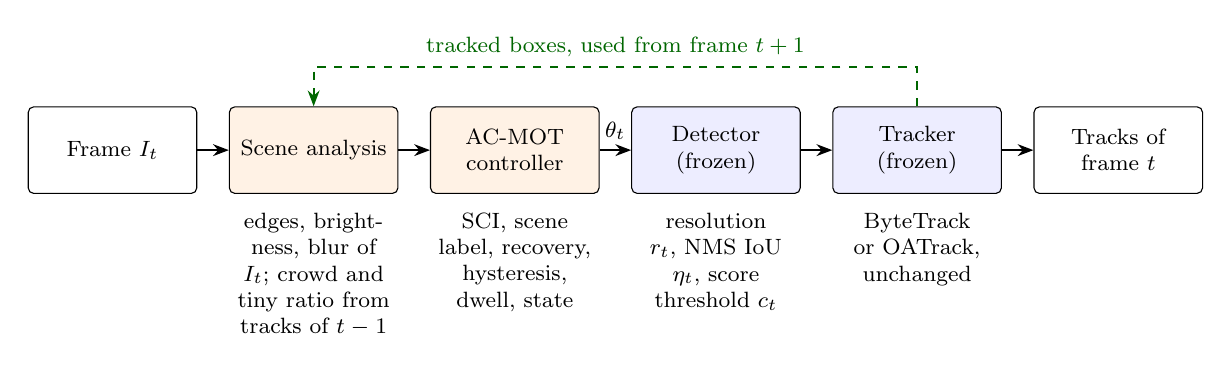
\begin{tikzpicture}[
  font=\footnotesize,
  node distance=4mm,
  stage/.style={draw, rounded corners=2pt, align=center, text width=20mm,
                minimum height=11mm, inner sep=2pt},
  ctrl/.style={stage, fill=orange!10},
  host/.style={stage, fill=blue!7},
  note/.style={align=center, text width=22.5mm, font=\footnotesize, inner sep=1pt},
  arr/.style={-{Stealth[length=2mm]}, thick},
  fb/.style={-{Stealth[length=2mm]}, thick, dashed, green!40!black}]
\node[stage] (frame) {Frame $I_t$};
\node[ctrl, right=of frame] (scene) {Scene analysis};
\node[ctrl, right=of scene] (ctrl) {AC-MOT\\controller};
\node[host, right=of ctrl] (det) {Detector\\(frozen)};
\node[host, right=of det] (trk) {Tracker\\(frozen)};
\node[stage, right=of trk] (out) {Tracks of\\frame $t$};
\draw[arr] (frame) -- (scene);
\draw[arr] (scene) -- (ctrl);
\draw[arr] (ctrl) -- node[above, font=\footnotesize] {$\theta_t$} (det);
\draw[arr] (det) -- (trk);
\draw[arr] (trk) -- (out);
\node[note, below=2mm of scene] {edges, brightness, blur of $I_t$; crowd and tiny ratio from tracks of $t-1$};
\node[note, below=2mm of ctrl] {SCI, scene label, recovery, hysteresis, dwell, state};
\node[note, below=2mm of det] {resolution $r_t$, NMS IoU $\eta_t$, score threshold $c_t$};
\node[note, below=2mm of trk] {ByteTrack or OATrack, unchanged};
\draw[fb] (trk.north) -- ++(0,5mm) -| node[pos=0.25, above, font=\footnotesize]
  {tracked boxes, used from frame $t+1$} (scene.north);
\end{tikzpicture}
\caption{AC-MOT in a tracking-by-detection pipeline. Scene analysis and the
controller choose the operating point $\theta_t=(c_t,\eta_t,r_t)$ before the
detector runs. The frozen detector and tracker are not modified. Tracked boxes
of frame $t$ feed the scene analysis of later frames (dashed arrow).}
\label{fig:pipeline}
\end{figure}


\subsection{Scene cues}\label{sec:cues}
The controller needs a cheap description of the scene. Scene analysis
therefore does not run on every frame. It runs on frame 1 and then once
every 10 frames ($t=1$ or $t \bmod 10 = 1$, that is, frames 1, 11, 21,
\dots). Each of these frames is an analysis step $j$. Between two analysis
steps the controller keeps its last decision. The stride of 10 frames is
selected by a temporal sweep on validation data that requires at least 25
FPS (Sec.~\ref{sec:constants}). Two kinds of cues are computed
at each step: image cues, which describe how the current frame looks, and box
cues, which describe the objects that the tracker found in the previous
frame.

\emph{Image cues of the current frame.} The frame is reduced to a quarter of
its width and height and converted to gray levels, so that the cues are cheap
to compute. Three cues are then measured:
\begin{itemize}
\item the edge density $e_t$, the fraction of pixels marked as edges by the
      Canny detector (lower and upper thresholds 50 and 120); many edges
      indicate a cluttered scene;
\item the brightness $\beta_t$, the mean gray level from 0 (black) to 255
      (white); a low value indicates a dark or night scene;
\item the sharpness $\nu_t$, the variance of the Laplacian of the gray image;
      a low value indicates a blurred frame.
\end{itemize}

\emph{Box cues of the previous frame.} Let $N_j$ be the number of boxes that
the tracker reported for frame $t-1$, and let $a_i$ be the area of box $i$ in
pixels of the original image. The crowd cue and the tiny-object ratio are
\begin{align}
C_j&=\min\!\left(\frac{N_j}{30},1\right),\label{eq:crowd}\\
T_j&=\frac{1}{N_j}\sum_{i=1}^{N_j}\mathbf{1}\!\left[a_i<32^2\right].\label{eq:tiny}
\end{align}
$C_j$ is the number of tracked objects divided by 30 and capped at 1, so every
frame with 30 or more objects has $C_j=1$. $T_j$ is the fraction of tracked
boxes smaller than $32\times32$ pixels, which is the size limit of small
objects in the COCO benchmark \cite{lin2014coco}. The indicator
$\mathbf{1}[\cdot]$ is 1 when its condition holds and 0 otherwise, and $T_j=0$
when $N_j=0$.

\subsection{SCI and scene label}\label{sec:sci}
The SCI measures how crowded the recent frames are.
A single frame is a noisy measurement, because the tracker may miss or add a
few objects in any frame, so the SCI averages over time. It is the mean crowd
cue of the last seven analysis steps:
\begin{equation}
S_j=\frac{1}{|H_j|}\sum_{k\in H_j} C_k,
\label{eq:sci}
\end{equation}
where $H_j$ holds the steps $j-6,\dots,j$ (fewer at the start of a video) and
$|H_j|$ is their number. With a stride of 10 frames, the seven steps cover
about the last 60 frames, so a single unusual frame changes $S_j$ only a little. The
window of seven steps is selected by the same temporal sweep as the stride
(Sec.~\ref{sec:constants}). Because $C_j\le1$, $S_j$ lies between 0 and 1.
While fewer than 30 objects are tracked, $S_j$ is simply the recent average
number of tracked objects divided by 30.

The SCI uses the crowd cue alone. During development, all 31 combinations of
the five cues (crowd, tiny ratio, edges, brightness, and blur) are tested as
SCI inputs on the calibration sequences, and the crowd cue alone is selected
(Sec.~\ref{sec:modern}). The other four cues are still used as checks on the
state, mainly through the scene label
\begin{equation}
\ell_j=\begin{cases}
\text{night}   & \text{if } \beta_t<80,\\
\text{blur}    & \text{else if } \nu_t<180,\\
\text{tiny}    & \text{else if } T_j>0.50,\\
\text{crowded} & \text{else if } C_j>0.65 \text{ or } e_t>0.13,\\
\text{clear}   & \text{otherwise.}
\end{cases}
\label{eq:label}
\end{equation}
The conditions are checked from top to bottom, and the first one that holds
gives the label. For example, $T_j>0.50$ means that more than half of the
tracked boxes are tiny, and $C_j>0.65$ means that at least 20 objects are
tracked.

Each cue therefore has a specific role. Only the crowd cue enters the SCI,
and it also enters the crowded label. The tiny-object ratio $T_j$ is used directly by the state rules of
Sec.~\ref{sec:states} and also gives the tiny label. The edge density $e_t$
is used only through the crowded label. The brightness $\beta_t$ and the
sharpness $\nu_t$ are used only through the night and blur labels. These two
labels do not lead to MEDIUM or HIGH by themselves. Because they are checked
first, their only effect is that a dark or blurred frame cannot receive the
crowded or tiny label; the SCI conditions and the tiny-object guard of
Eq.~\eqref{eq:target} still apply to such a frame.

\subsection{Three-state controller}\label{sec:states}
The controller is always in one of three states: LOW, MEDIUM, or HIGH. The
names describe the scene: LOW for a sparse scene, HIGH for a crowded scene or
a scene of mostly tiny objects. They do not rank the input size: in the final
action map the HIGH state uses the smallest input (Table~\ref{tab:actions}).
The state is updated only at analysis steps, in four steps
(Algorithm~\ref{alg:controller}). Step~1 proposes a target state from the
cues. Steps~2--4 adjust this target so that the controller reacts to a sudden
drop in the object count but does not switch back and forth.

\emph{Step 1: target state.} The target is the state that the current cues
ask for. It is given by the SCI, the tiny-object ratio, and the scene label:
\begin{equation}
g_j=\begin{cases}
\text{HIGH}   & \text{if } S_j>\tau_h \text{ or } T_j>0.50,\\
\text{MEDIUM} & \text{else if } S_j>\tau_m \text{ or}\\
              & \quad \ell_j\in\{\text{crowded},\text{tiny}\},\\
\text{LOW}    & \text{otherwise,}
\end{cases}
\label{eq:target}
\end{equation}
where $\tau_m=0.297$ and $\tau_h=0.511$ are the two SCI thresholds
(Table~\ref{tab:constants}). They are selected by the joint search
on the calibration sequences (Sec.~\ref{sec:constants}). Since $S_j$ is the
recent average number of tracked objects divided by 30, the SCI conditions
give MEDIUM above about 9 objects ($30\tau_m=8.9$) and HIGH above about 15
objects ($30\tau_h=15.3$).

\emph{Step 2: recovery probe.} The SCI averages seven steps, so it reacts
slowly when the tracker suddenly reports far fewer objects than a few steps
earlier. The recovery probe responds to such a collapse of the object count.
Instead of letting the falling count move the controller toward a lower
state, it sets the target to HIGH for a short time. To detect a collapse, it
keeps a slowly decaying peak $P_j$ of the object count and a drop counter
$d_j$:
\begin{align}
d_j&=\begin{cases}
d_{j-1}+1 & \text{if } P_{j-1}\ge5 \text{ and}\\
          & \quad N_j<0.40\,P_{j-1},\\
0         & \text{otherwise,}
\end{cases}\label{eq:drop}\\
P_j&=\max\left(N_j,\lfloor 0.8\,P_{j-1}\rfloor\right),\label{eq:peak}
\end{align}
with $P_0=d_0=0$. A collapse is detected when at least 5 objects have been seen
before and fewer than 40\% of them remain. The peak loses 20\% at each step,
so an old peak is forgotten after a few steps. While $1\le d_j\le3$, the
target $g_j$ is set to HIGH, so the probe lasts at most three analysis steps
(30 frames); the dwell rule of Step~4 still applies. The rule and its values
come from the original AC-MOT controller and are fixed in all final-stage
searches (Sec.~\ref{sec:constants}), so the HIGH action used during a probe
is selected by the joint search with this rule in place.

\emph{Step 3: hysteresis.} Without a margin, a scene whose SCI stays close to
a threshold would make the controller switch at almost every step.
Hysteresis prevents this: a move to a lower state is held while the scene is
still close to difficult:
\begin{equation}
g_j\leftarrow\begin{cases}
\text{HIGH}   & \text{if } q_{j-1}=\text{HIGH} \text{ and}\\
              & \quad (S_j>0.50 \text{ or } T_j>0.40),\\
\text{MEDIUM} & \text{if } q_{j-1}=\text{MEDIUM},\\
              & \quad g_j=\text{LOW} \text{ and } S_j>0.25,\\
g_j           & \text{otherwise.}
\end{cases}
\label{eq:hold}
\end{equation}
The hold values lie just below the values that lead into each state
($0.50<\tau_h$, 0.40 below the tiny guard of 0.50, and $0.25<\tau_m$).
Upward moves are not held.

\emph{Step 4: dwell.} The dwell rule sets a minimum time between two changes.
After a change, the state is kept for at least 30 frames, that is, three
analysis steps:
\begin{equation}
q_j=\begin{cases}
g_j     & \text{if } t-t_c\ge30,\\
q_{j-1} & \text{otherwise,}
\end{cases}
\label{eq:dwell}
\end{equation}
where $t_c$ is the frame of the last state change. The controller starts in
LOW with $t_c=1$, so the first change is possible at frame 31. Whenever
$q_j\ne q_{j-1}$, $t_c$ is set to $t$.

\emph{Why changes are kept rare.} Each change of state changes the input size
and the thresholds, and thus the boxes that reach the tracker. Apart from the
recovery probe, the temporal rules let the state follow lasting changes of
the scene, not single frames: the seven-step window smooths the SCI over about
60 frames, the holds add a margin below each threshold, and the dwell rule
allows at most one change every 30 frames.

\emph{Example.} Consider a clear, sharp video in which the tracker reports 20
objects of normal size in every frame ($C_j=0.67$), and only 10 objects from
frame 71 on. The controller starts in LOW. The first step sees no earlier
boxes ($C_j=0$), so $S_j$ grows as the window fills: 0.33 at frame 11, 0.44
at frame 21, and 0.50 at frame 31. The target is MEDIUM from frame 11, but the
dwell rule keeps LOW until frame 31, where the state becomes MEDIUM. From
frame 41, $S_j$ exceeds $\tau_h$ and the target is HIGH; the dwell rule delays
this change to frame 61. When the scene thins, $S_j$ falls slowly because the
window still holds the earlier steps, so the state stays HIGH until frame 101.
At frame 111, $S_j=0.48$ is below both $\tau_h$ and the hold value of 0.50,
and the state returns to MEDIUM. It then stays in MEDIUM, because 10 tracked
objects keep $S_j$ at about 0.33, above $\tau_m$.

The state $q_j$ then selects the operating point from the action map, and the
detector uses it until the next analysis step.

\begin{algorithm}[htbp]
\caption{AC-MOT controller for one video}\label{alg:controller}
\begin{algorithmic}[1]
\State $j\gets0$; $q_0\gets$ LOW; $P_0\gets0$; $d_0\gets0$; $t_c\gets1$
\For{each frame $t=1,2,\dots$}
  \If{$t=1$ \textbf{or} $t \bmod 10=1$}
    \State $j\gets j+1$
    \State $e_t,\beta_t,\nu_t\gets$ image cues of $I_t$
    \State $N_j,C_j,T_j\gets$ box cues of frame $t-1$ (Eqs.~\ref{eq:crowd}--\ref{eq:tiny})
    \State $S_j\gets$ mean of $C$ over $H_j$, the last 7 steps (Eq.~\ref{eq:sci})
    \State $\ell_j\gets$ label (Eq.~\ref{eq:label}); $g_j\gets$ target (Eq.~\ref{eq:target})
    \State update $d_j$ and $P_j$ (Eqs.~\ref{eq:drop}--\ref{eq:peak})
    \If{$1\leq d_j\leq3$} $g_j\gets$ HIGH
    \EndIf
    \State apply the holds to $g_j$ (Eq.~\ref{eq:hold})
    \If{$t-t_c\geq30$ \textbf{and} $g_j\neq q_{j-1}$}
      \State $q_j\gets g_j$; $t_c\gets t$
    \Else
      \State $q_j\gets q_{j-1}$
    \EndIf
  \EndIf
  \State $(r_t,\eta_t,c_t)\gets$ action of state $q_j$ (Table~\ref{tab:actions})
  \State detect with $r_t$ and $\eta_t$; drop boxes with score $<c_t$
  \State update the tracker; store its boxes of frame $t$
\EndFor
\end{algorithmic}
\end{algorithm}

\subsection{Action map}\label{sec:actions}
Table~\ref{tab:actions} gives the operating point of each state. The actions
are not set by hand: they are selected together with $\tau_m$ and $\tau_h$
by the joint search on the calibration sequences, whose objective is the
change in HOTA, a metric that balances detection and association
(Sec.~\ref{sec:constants}).

LOW uses the largest input (1536 pixels), loose NMS (0.70), and a low score
threshold (0.10), so the detector passes more weak boxes when the scene is
sparse. MEDIUM uses 1280 pixels, tight NMS (0.45), and a score threshold of
0.40. HIGH uses 1088 pixels, NMS 0.60, and a score threshold of 0.40. In the
two difficult states, the detector therefore passes only boxes with a score of
at least 0.40.

The HIGH state, used for crowded scenes and for scenes of mostly tiny objects,
thus has the smallest input and a high score threshold. This may look
surprising, since a larger input shows small objects better. The search,
however, optimizes tracking quality, not the detection of every small object.
A score threshold of 0.40 gives the tracker fewer but more reliable boxes; in
a separate sweep of fixed score thresholds on the same sequences, at 1088
pixels and NMS 0.45, 0.40 gives the highest pooled HOTA
(Sec.~\ref{sec:constants}). The smaller input also
costs less detector time. Section~\ref{sec:results} shows that the main effect
of AC-MOT is a more selective detection stream: fewer FP and
IDS, with similar or slightly lower recall. This action is the
result of the search, not a general rule that crowded scenes need smaller
inputs.

The score threshold $c_t$ is applied on the detector side before the tracker.
It is separate from any confidence gate inside the tracker, such as the fixed
tracker-side gate of OATrack.

\begin{table}[htbp]
\caption{Action map. State names describe scene difficulty, not a resolution
rank. Selected by the joint search on the calibration sequences.}
\label{tab:actions}
\centering\footnotesize
\begin{tabular}{@{}lrrr@{}}
\toprule
State & Resolution $r$ & NMS IoU $\eta$ & Score threshold $c$\\
\midrule
LOW & 1536 & 0.70 & 0.10\\
MEDIUM & 1280 & 0.45 & 0.40\\
HIGH & 1088 & 0.60 & 0.40\\
\bottomrule
\end{tabular}
\end{table}

\subsection{Selection of Parameter Values of the AC-MOT Controller}\label{sec:constants}
All values of Tables~\ref{tab:actions} and~\ref{tab:constants} are fixed
before the final evaluation and are not changed after it. The last column of
Table~\ref{tab:constants} gives the source of each value. There are four
sources.

\emph{Joint search on the calibration sequences.} The SCI thresholds $\tau_m$
and $\tau_h$ and the action map are selected together by an Optuna TPE search
with 60 trials \cite{akiba2019optuna}; the search ranges are given in
Sec.~\ref{sec:modern}. The calibration sequences are eight
sequences of the VisDrone2019-MOT training split. They serve as the validation
(tuning) data of the final stage and are disjoint from the evaluation
sequences. Each trial is scored by four-fold cross-validation, with two
sequences held out in each fold, as the mean change in HOTA against the
baseline. The candidate values come from existing settings. The input sizes
(1088, 1280, and 1536 pixels) and NMS values (0.45, 0.60, and 0.70) are the
operating points for which detector outputs are cached; 1536 pixels
with NMS 0.70 is the baseline point, and 0.70 is the default NMS value of the
Ultralytics detector. The three score thresholds are the low and high
thresholds of ByteTrack (0.10 and 0.25) and the confidence gate of OATrack
(0.40). In a separate sweep of the score threshold over 0.01, 0.10, 0.25, and
0.40 on the same sequences, at 1088 pixels and NMS 0.45, 0.40 gives the highest
pooled HOTA (+0.881 over 0.01) and improves seven of the eight sequences. The frozen policy reaches a mean HOTA
gain of 2.447 points over the four folds, with all folds positive
(Sec.~\ref{sec:modern}).

\emph{Cue audit on the calibration sequences.} The choice of the crowd cue as
the only SCI input comes from testing all 31 non-empty subsets of the five
cues with the same cross-validation (Sec.~\ref{sec:modern}).

\emph{Temporal sweep on the validation split.} The analysis stride and the
SCI window are selected in the first development stage, with the YOLOv8n
pipeline, on the VisDrone2019-MOT validation sequences. The sweep tests 25
combinations: windows of 1, 3, 5, 7, and 9 analysis steps and strides of 1, 5,
10, 15, and 20 frames. Five of the 25 settings meet both constraints of that
stage, at least 25 FPS and at most 271 IDS (the IDS of the original controller
on the same data). Among them, a window of 7 and a stride of 10 give the
highest MOTA, 18.165 against 18.044 for the next setting. Operating-point
sweeps on the same data cover input resolutions from 512 to 960 pixels,
confidence thresholds from 0.05 to 0.50, and NMS thresholds from 0.30 to 0.80,
and define the supported values of the first optimized profiles
(Sec.~\ref{sec:development}).

\emph{Fixed design values.} The tiny-object area follows the COCO definition
of small objects \cite{lin2014coco}. The remaining values (the crowd
normalizer, the Canny thresholds, the label thresholds, the recovery, hold,
and dwell values, and the initial state) come from the original AC-MOT
controller and are kept unchanged in every search of the final stage. The
searched values above
are tuned with these values in place, so the selected thresholds and actions
are matched to them. For example, the crowd normalizer of 30 only sets the
scale of $S_j$: $\tau_m$ and $\tau_h$ are searched on this scale and
correspond to about 9 and 15 tracked objects.

\begin{table}[htbp]
\caption{Values of the AC-MOT controller and how each value is chosen.
Calibration sequences: eight VisDrone2019-MOT training sequences used as
tuning data, disjoint from the evaluation sequences. CV: four-fold
cross-validation.}
\label{tab:constants}
\centering\footnotesize
\setlength{\tabcolsep}{4pt}
\begin{tabular}{@{}l>{\raggedright\arraybackslash}p{50mm}l>{\raggedright\arraybackslash}p{62mm}@{}}
\toprule
Symbol & Meaning & Value & How the value is chosen\\
\midrule
$\tau_m$ & SCI threshold for MEDIUM, Eq.~\eqref{eq:target} & 0.297 & joint TPE search on the calibration sequences, 60 trials, CV\\
$\tau_h$ & SCI threshold for HIGH, Eq.~\eqref{eq:target} & 0.511 & same joint search\\
$(r,\eta,c)$ & operating point of each state & Table~\ref{tab:actions} & same joint search over $\{1088,1280,1536\}\times\{0.45,0.60,0.70\}\times\{0.10,0.25,0.40\}$\\
-- & SCI input cue & crowd only & cue audit of all 31 cue subsets on the calibration sequences, CV\\
-- & analysis stride & 10 frames & temporal sweep of 25 settings on the validation split; highest MOTA with $\geq$25 FPS and $\leq$271 IDS\\
$|H_j|$ & SCI window & 7 steps & same temporal sweep\\
-- & tiny-object area & $32\times32$ pixels & COCO small-object limit \cite{lin2014coco}\\
-- & crowd normalizer, Eq.~\eqref{eq:crowd} & 30 boxes & original controller; sets the scale on which $\tau_m$, $\tau_h$ are searched\\
-- & Canny thresholds (lower, upper) & 50, 120 & original controller; fixed in all final-stage searches\\
-- & night and blur labels, Eq.~\eqref{eq:label} & $\beta_t<80$, $\nu_t<180$ & original controller; fixed in all final-stage searches\\
-- & crowded label, Eq.~\eqref{eq:label} & $C_j>0.65$ or $e_t>0.13$ & original controller; fixed in all final-stage searches\\
-- & tiny label and HIGH guard, Eqs.~\eqref{eq:label}, \eqref{eq:target} & $T_j>0.50$ & original controller; fixed in all final-stage searches\\
-- & recovery: minimum peak, drop ratio, peak decay, steps & 5, 0.40, 0.80, 3 & original controller; fixed in all final-stage searches\\
-- & holds in HIGH ($S_j$, $T_j$) and MEDIUM ($S_j$), Eq.~\eqref{eq:hold} & (0.50, 0.40), 0.25 & original controller; fixed in all final-stage searches\\
-- & dwell, Eq.~\eqref{eq:dwell} & 30 frames & original controller; fixed in all final-stage searches\\
-- & initial state & LOW & original controller; fixed in all final-stage searches\\
\bottomrule
\end{tabular}
\end{table}
\section{Development of the Final AC-MOT Controller}\label{sec:development}

The controller of Sec.~\ref{sec:method} is the result of four development
stages, and each stage asked one question. The quality-oriented profile
(Sec.~\ref{sec:quality}) asked whether a scene index that steers the detector
settings can improve tracking over a fixed default operating point. The
identity-aware profile (Sec.~\ref{sec:identity}) asked what changes when
identity stability and speed are explicit objectives. The transfer studies
(Sec.~\ref{sec:transfer}) asked whether these profiles keep their effect on
other data and pipelines. The modern stage (Sec.~\ref{sec:modern}) asked how
the controller should be built for a modern detector with separate
calibration data, and produced the frozen controller.

The first three stages are historical. Their controllers differ from the
final one: the two profiles used a weighted five-cue index with interpolated
confidence and NMS values and three resolution levels, and the SparseTrack
study used a single edge-driven NMS rule. They also used other detectors and
evaluation protocols. Their numbers are therefore reported in their own
tables, each against its own baseline, and are not pooled with the modern
results. The end of each stage states what it showed.

\subsection{Quality-oriented profile}\label{sec:quality}

\emph{Baseline.} The reference pipeline is the pretrained YOLOv8n detector
\cite{jocher2023yolov8} followed by ByteTrack \cite{zhang2022bytetrack}, both at
their default settings: confidence threshold 0.25, NMS IoU threshold 0.45,
input size 640 pixels, and the default ByteTrack parameters (high threshold
0.25, low threshold 0.10, new-track threshold 0.25, buffer 30 frames, match
threshold 0.80). It runs with one fixed operating point for the whole video.

\emph{Method.} The first optimization-derived profile kept the same detector,
used a tuned ByteTrack profile, and searched only on the VisDrone2019-MOT
validation split. Five cues were used: crowd count, the fraction of earlier
boxes below $32\times32$ pixels, edge density, low brightness, and low
Laplacian variance. Each cue was normalized with validation statistics, and
the index was their weighted sum
\begin{equation}
S_j=\sum_{k\in\{c,t,e,n,b\}}w_k\,x_{k,j},
\label{eq:hist-sci}
\end{equation}
where $k$ runs over the five cues (c: crowd, t: tiny ratio, e: edges, n: low
brightness, b: blur), $x_{k,j}$ is the normalized value of cue $k$ at analysis
step $j$, and $w_k$ is its weight, with $w_k\geq0$ and $\sum_k w_k=1$. The
index was averaged over seven analyses taken every ten frames. Confidence and NMS were interpolated linearly between the values
at $S=0$ and $S=1$, and two sorted thresholds selected one of three
resolutions (512, 928, 960 pixels).

An Optuna TPE study \cite{akiba2019optuna} jointly searched the five weights,
the confidence and NMS end points, and the two thresholds. The resolution
levels, the supported confidence values $\{0.25,\dots,0.45\}$, the supported
NMS values from 0.30 to 0.70, and the temporal settings were fixed beforehand
by validation sweeps (Sec.~\ref{sec:constants}). The selection rule kept
trials with at least 25 FPS and at most 271 IDS (the IDS of the original
controller on the same validation data) and then took the highest MOTA, with lower IDS, HOTA,
IDF1, and FPS as tie-breaks. The frozen profile (archived as Trial~24) has
$w_c=0.1294928$, $w_t=0.2217477$, $w_e=0.4337134$, $w_n=0.0535577$,
$w_b=0.1614885$, confidence end points $(0.30,0.40)$, NMS end points
$(0.35,0.35)$, and thresholds $(0.1353494, 0.2872868)$. On validation it
reached MOTA 23.038, HOTA 36.110, IDF1 40.758, and IDS 270 at 37.169 FPS.

\emph{Comparison.} Table~\ref{tab:quality} compares the profile with the
baseline on the historical VisDrone test-dev split, with paired bootstrap
intervals (5000 resamples, seed 42). HOTA rises by 5.4051 points, MOTA by
7.2195 points, and IDF1 by 8.8220 points, and throughput rises from 36.528 to
38.985 FPS.

\emph{What this stage showed.} A scene index that steers the detector settings
improved tracking quality over the fixed default point, with HOTA, MOTA, and
IDF1 intervals above zero. The IDS interval, $[-114, 219]$, includes zero; the
next stage made identity stability an explicit objective. The final
controller keeps two parts of this stage: the stride of 10 frames and the
window of seven steps from its temporal sweep (Sec.~\ref{sec:constants}), and
the five kinds of scene cues, which were audited again in the modern stage.

\begin{table}[htbp]
\caption{Quality-oriented profile versus its baseline (YOLOv8n with ByteTrack
at default settings) on VisDrone test-dev, historical protocol. Gain: paired
bootstrap difference with 95\% interval; for IDS it is the reduction.}
\label{tab:quality}
\centering\footnotesize
\setlength{\tabcolsep}{4pt}
\begin{tabular}{@{}lrrl@{}}
\toprule
Metric & Baseline & Quality & Gain [95\% CI]\\
\midrule
HOTA & 28.430 & 33.835 & $+5.4051$ $[4.1273, 6.9022]$\\
MOTA & 19.729 & 26.948 & $+7.2195$ $[5.4362, 9.2934]$\\
IDF1 & 32.724 & 41.546 & $+8.8220$ $[6.9005, 11.0537]$\\
IDS & 1235 & 1184 & $51$ $[-114, 219]$\\
FPS & 36.528 & 38.985 & --\\
\bottomrule
\end{tabular}
\end{table}

\subsection{Identity-aware Pareto profile}\label{sec:identity}

\emph{Baseline.} The baseline is the same YOLOv8n and ByteTrack pipeline at
default settings (Sec.~\ref{sec:quality}).

\emph{Method.} Quality is not the only deployment goal; identity stability and
compute can move in a different direction from MOTA. The second study kept
the same cues, operating levels, temporal settings, and validation data, but
changed the question. It maximized MOTA and minimized IDS subject only to
$\mathrm{FPS}\geq25$, without the IDS gate. A seeded TPE sampler ran 49
completed trials. A trial dominated another when it had no lower MOTA and no
higher IDS, with at least one strict improvement, and the feasible Pareto
front was built from these relations. The balanced
candidate maximized an equal-weight score of normalized MOTA and normalized IDS
reduction, with HOTA, IDF1, FPS, and trial index as tie-breaks.

The selected profile (archived as Trial~22) has weights $w_c=0.1646453$,
$w_t=0.1746265$, $w_e=0.5076113$, $w_n=0.1206956$, $w_b=0.0324213$,
confidence end points $(0.40,0.40)$, NMS end points $(0.60,0.35)$, and
thresholds $(0.2927136, 0.6661672)$. On validation it reached MOTA 19.330,
HOTA 31.651, IDF1 34.226, and IDS 168 at 51.406 FPS.

\emph{Comparison.} Table~\ref{tab:identity} compares the profile with the
baseline on test-dev. It removes 316 IDS and raises throughput
from 36.528 to 46.024 FPS, while HOTA, MOTA, and IDF1 also rise. Against the
quality-oriented profile it has 265 fewer IDS $[82, 502]$ and $-2.617$ HOTA
$[-4.004, -1.694]$. The two profiles therefore answer different questions: one
favors overall quality and the other favors identity stability and speed.

\emph{What this stage showed.} The detector operating point controls a
trade-off between quality, identity stability, and speed, and the objective
of the search decides which side is favored. The next stage tested whether
such profiles keep their effect outside the data and pipeline on which they
were tuned.

\begin{table}[htbp]
\caption{Identity-aware profile versus its baseline (YOLOv8n with ByteTrack at
default settings) on VisDrone test-dev, historical protocol. Gain: paired
bootstrap difference with 95\% interval; for IDS it is the reduction.}
\label{tab:identity}
\centering\footnotesize
\setlength{\tabcolsep}{4pt}
\begin{tabular}{@{}lrrl@{}}
\toprule
Metric & Baseline & Identity & Gain [95\% CI]\\
\midrule
HOTA & 28.430 & 31.218 & $+2.788$ $[0.747, 4.660]$\\
MOTA & 19.729 & 23.792 & $+4.063$ $[0.952, 6.886]$\\
IDF1 & 32.724 & 37.870 & $+5.146$ $[2.028, 8.080]$\\
IDS & 1235 & 919 & $316$ $[175, 470]$\\
FPS & 36.528 & 46.024 & --\\
\bottomrule
\end{tabular}
\end{table}

\subsection{Transfer and cross-pipeline studies}\label{sec:transfer}

This stage applied the historical controllers outside their development
setting: to a second dataset, and to two other detector--tracker pipelines.

\emph{UAVDT.} The baseline is again YOLOv8n with ByteTrack at default settings
(Sec.~\ref{sec:quality}). Both frozen profiles were applied to UAVDT
\cite{du2018uavdt} without retuning (Table~\ref{tab:hist-uavdt}). The
quality-oriented profile raised HOTA by 4.305 points $[2.740, 5.709]$ and the
identity-aware profile by 2.845 points $[1.238, 4.348]$; their IDS reductions
are 237 $[104, 377]$ and 250 $[110, 404]$.

\begin{table}[htbp]
\caption{Historical UAVDT transfer without retuning. Baseline: YOLOv8n with
ByteTrack at default settings.}
\label{tab:hist-uavdt}
\centering\footnotesize
\setlength{\tabcolsep}{4pt}
\begin{tabular}{@{}lrrr@{}}
\toprule
Metric & Baseline & Quality & Identity\\
\midrule
HOTA & 24.085 & 28.390 & 26.930\\
MOTA & 13.841 & 17.399 & 16.118\\
IDF1 & 27.887 & 34.453 & 32.014\\
IDS & 558 & 321 & 308\\
FPS & 65.015 & 58.353 & 61.462\\
\bottomrule
\end{tabular}
\end{table}

\emph{U2MOT on VisDrone.} The baseline is the published U2MOT tracker
\cite{liu2023u2mot} with its released YOLOX-X detector, run
at its own static setting. Seven VisDrone validation sequences served for
development and 17 test-dev sequences for evaluation. The cue weights and
transforms of the quality-oriented profile were kept, the tracker was not
modified, and the action boundaries were set to the 33rd and 67th percentiles
of the index on the U2MOT validation run, without using ground truth.
Table~\ref{tab:u2mot} gives the comparison: the controlled pipeline has 87
fewer IDS and 1230 fewer FP, while MOTA is almost unchanged and FN are higher.

\begin{table}[htbp]
\caption{Cross-pipeline study on VisDrone test-dev. Baseline: U2MOT with its
YOLOX-X detector at its static setting.}
\label{tab:u2mot}
\centering\footnotesize
\setlength{\tabcolsep}{4pt}
\begin{tabular}{@{}lrr@{}}
\toprule
Metric & U2MOT baseline & With controller\\
\midrule
MOTA & 53.873 & 53.767\\
IDF1 & 69.775 & 69.849\\
IDS & 1239 & 1152\\
FP & 41385 & 40155\\
FN & 63241 & 64801\\
\bottomrule
\end{tabular}
\end{table}

\emph{SparseTrack on MOT17.} The baseline is the published SparseTrack tracker
\cite{liu2025sparsetrack} with a fixed NMS IoU threshold of 0.75, on the seven
MOT17 \texttt{val\_half} sequences (2652 frames) \cite{dendorfer2021motchallenge}.
A minimal edge-driven rule switched only the NMS threshold, between 0.70 and
0.80; its threshold came from a leave-one-sequence-out study on the same
sequences. Table~\ref{tab:sparsetrack} gives the comparison: the adaptive rule
reduces IDS from 136 to 123, with MOTA $+0.0371$ points $[-0.041, +0.182]$.

\begin{table}[htbp]
\caption{Cross-pipeline study on MOT17 \texttt{val\_half}. Baseline:
SparseTrack with a fixed NMS IoU threshold of 0.75.}
\label{tab:sparsetrack}
\centering\footnotesize
\setlength{\tabcolsep}{4pt}
\begin{tabular}{@{}lrr@{}}
\toprule
Metric & SparseTrack baseline & With adaptive NMS\\
\midrule
MOTA & 76.8881 & 76.9252\\
IDF1 & 81.4943 & 81.5299\\
IDS & 136 & 123\\
\bottomrule
\end{tabular}
\end{table}

\emph{What this stage showed.} The frozen profiles kept their direction on
UAVDT without retuning, and with U2MOT and SparseTrack the control mainly
reduced IDS, with small changes in MOTA. Together these
studies show that the preferred profile depends on the objective (quality or
identity) and on the tracker host. This motivated a modern stage with a
stronger detector, explicit calibration data, and two tracker hosts.

\subsection{Modern development of the frozen controller}\label{sec:modern}

The modern stage started from the scene cues and state logic of the original
controller and decided, step by step, which cues enter the SCI, which
operating points each state uses, and where the SCI thresholds lie.

\emph{Baseline.} The modern baseline is the YOLO11m detector
\cite{jocher2024yolo11}, in the public VisDrone checkpoint described in
Sec.~\ref{sec:hosts}, run at a fixed operating point of 1536 pixels and NMS
IoU 0.70 with no extra score threshold. It feeds ByteTrack
\cite{zhang2022bytetrack} during development and both ByteTrack and OATrack
\cite{qi2026oatrack} in the final evaluation. A large fixed input is a common
choice for small aerial objects when no adaptation is used.

\emph{Data and protocol.} Eight sequences of the VisDrone2019-MOT training split
(3282 frames) were declared as calibration data. They are disjoint from the
seven evaluation sequences. The searches used the same four folds, each
holding out two calibration sequences. Detector outputs were cached for
every resolution and NMS value; a score threshold applied to the cache was
checked to reproduce direct inference exactly. Table~\ref{tab:devrecord}
summarizes the development steps, which are described below in the order in
which they were carried out.

\emph{Resolution and NMS maps.} Two exhaustive grid searches, archived as
Stages 1 and 2, searched the state-to-resolution and state-to-NMS maps. At
this point the action of a state contained only the input resolution and the
NMS value.

\emph{Cue audit.} The next search, archived as Stage 3A, asked which cues
should form the SCI. It searched
all 31 non-empty subsets of the five cues and selected \{crowd\}, which defines
the crowd-selected SCI of Eq.~\eqref{eq:sci}. The other cues were kept as guard
and auxiliary cues of the state logic (Sec.~\ref{sec:sci}).

\emph{Score threshold.} A separate sweep then tested the score threshold. At
1088 pixels and NMS 0.45, a fixed score threshold of 0.40 raised pooled
calibration HOTA by $+0.881$ over 0.01 and improved seven of the eight
sequences. The score threshold was therefore added as the third action
dimension.

\emph{Final joint search.} The final search then selected the thresholds and
the three-part actions together. It used 60 TPE trials (seed 43) and searched
$\tau_m\in[0.10,0.50]$, $\tau_h\in[\tau_m+0.05,\min(\tau_m+0.40,0.90)]$,
and for each state a resolution in $\{1088,1280,1536\}$, an NMS value in
$\{0.45,0.60,0.70\}$, and a score threshold in $\{0.10,0.25,0.40\}$. The
objective was the cross-validated (CV) mean change in HOTA against the
baseline, with ByteTrack as host. A candidate was eligible only if it really adapted within the video
rather than acting as one fixed operating point: it had to realize at least
two distinct actions, each on at least 10\% of calibration frames, and switch
within sequences. The frozen policy is the eligible candidate whose three
states use three different actions that together vary all three parts of the
operating point (Table~\ref{tab:actions}). On calibration data it used LOW,
MEDIUM, and HIGH on 7.6\%, 10.1\%, and 82.3\% of frames, with 0.607 state
changes per 100 frames on average.

\emph{Comparison.} Table~\ref{tab:folds} compares the frozen policy with the
baseline on each calibration fold. All four folds are positive, with a CV
mean of $+2.447$ HOTA. After these steps the thresholds, cue subset, and
action map were frozen. Compared with the historical profiles, the final
controller is simpler: one crowd index instead of a weighted five-cue index,
and three fixed actions instead of interpolated confidence and NMS values. The final
comparison on the evaluation sequences is given in Sec.~\ref{sec:results}.

\begin{table}[htbp]
\caption{Main modern development steps on the eight calibration sequences
(ByteTrack host). The score-threshold gain is pooled HOTA; the joint-search
result is the mean over four folds.}
\label{tab:devrecord}
\centering\footnotesize
\setlength{\tabcolsep}{3pt}
\begin{tabular}{@{}lll@{}}
\toprule
Step & Search & Result\\
\midrule
Cue subset & 31 subsets & \{crowd\}\\
Score threshold & 4 values & 0.40; $+0.881$ HOTA\\
Joint search & 60 TPE trials & CV mean $+2.447$\\
\bottomrule
\end{tabular}
\end{table}

\begin{table}[htbp]
\caption{Frozen policy versus the modern baseline (YOLO11m at 1536 pixels and
NMS 0.70, ByteTrack) on the four calibration folds: change in HOTA.}
\label{tab:folds}
\centering\footnotesize
\begin{tabular}{@{}lrrrrr@{}}
\toprule
 & Fold 1 & Fold 2 & Fold 3 & Fold 4 & Mean\\
\midrule
$\Delta$HOTA & $+0.592$ & $+4.164$ & $+2.029$ & $+3.004$ & $+2.447$\\
\bottomrule
\end{tabular}
\end{table}
\section{Results}\label{sec:results}

The experiments ask one question: with the same detector and the same
tracker, does replacing the fixed operating point by the frozen AC-MOT
controller improve tracking? The VisDrone evaluation answers this on the
dataset used for development, and the UAVDT transfer answers it on a second
dataset without any retuning.

All experiments use the YOLO11m detector of Sec.~\ref{sec:hosts}. It runs in
half precision, and detections of the classes pedestrian, car, van, truck, and
bus are passed on. ByteTrack uses the Ultralytics implementation with its
default parameters: high threshold 0.25, low threshold 0.10, new-track
threshold 0.25, buffer 30 frames, and match threshold 0.80. OATrack is a
re-implementation of the published method \cite{qi2026oatrack} in its main
configuration, with its published tracker-side confidence gate of 0.40. This
gate belongs to the tracker and is never changed by AC-MOT. For each host, two
systems are compared. The baseline runs the detector at the fixed operating
point of 1536 pixels and NMS IoU 0.70, with a minimal score threshold of 0.01.
This is the largest input of the operating-point grid, and 0.70 is the default
NMS value of the Ultralytics detector. AC-MOT runs the frozen controller of
Sec.~\ref{sec:method} on the same detector. The two systems differ only in
the detector operating point. Uncertainty is estimated with the paired
bootstrap of Sec.~\ref{sec:metrics}, with 5000 resamples (seed 42).
Latency is measured on one Tesla T4 GPU over the first 200 frames of sequence
\texttt{uav0000086\_00000\_v}, excluding five warm-up frames. For every
frame, the time spent in the controller (image statistics, scene analysis, and
state update) is recorded separately from the detector and tracker time.

\subsection{Frozen VisDrone evaluation}
The VisDrone evaluation uses seven sequences of the VisDrone2019-MOT
validation split. They contain 71,830 ground-truth boxes. The cue subset,
thresholds, and action map of the frozen controller were selected on the
separate calibration sequences only (Sec.~\ref{sec:modern}). Results are
scored with a Python port of the VisDrone2019-MOT Task~4b evaluation. Ignored
regions are removed, the five classes above are evaluated separately,
CLEAR-MOT and identity measures use IoU 0.5, and counts are summed over
classes and sequences. HOTA is added with the same class-aware scheme using
TrackEval. The bootstrap draws seven sequences with replacement.

Table~\ref{tab:visdrone} lists the aggregate results on the seven VisDrone
sequences, and Fig.~\ref{fig:visdrone} shows HOTA, MOTA, and IDF1.

\begin{table}[htbp]
\caption{Frozen VisDrone evaluation on seven VisDrone2019-MOT sequences
(71,830 ground-truth boxes). Baseline: fixed operating point (1536, 0.70).}
\label{tab:visdrone}
\centering\footnotesize
\setlength{\tabcolsep}{4pt}
\begin{tabular}{@{}lrrrr@{}}
\toprule
 & \multicolumn{2}{c}{ByteTrack} & \multicolumn{2}{c}{OATrack}\\
\cmidrule(lr){2-3}\cmidrule(l){4-5}
Metric & Baseline & AC-MOT & Baseline & AC-MOT\\
\midrule
HOTA & 41.586 & 44.523 & 46.770 & 48.095\\
MOTA & 9.876 & 27.871 & 28.165 & 34.483\\
IDF1 & 48.569 & 53.929 & 57.107 & 59.364\\
IDS & 1341 & 1016 & 773 & 604\\
FP & 39274 & 24892 & 25394 & 21400\\
FN & 24121 & 25902 & 25432 & 25057\\
Precision & 54.849 & 64.852 & 64.628 & 68.609\\
Recall & 66.419 & 63.940 & 64.594 & 65.116\\
\bottomrule
\end{tabular}
\end{table}

\emph{ByteTrack host.} AC-MOT changes HOTA from 41.586 to 44.523, MOTA from
9.876 to 27.871, and IDF1 from 48.569 to 53.929. IDS fall from 1341 to 1016
and FP from 39274 to 24892, while FN rise from 24121 to 25902. Precision rises
from 54.849 to 64.852 and recall falls from 66.419 to 63.940. The detector
output becomes more selective: clutter and identity-confusing boxes are
removed at a small cost in recall. The very low baseline MOTA shows how many
FP the fixed operating point passes to this tracker. Because
MOTA counts every FP, the removal of more than a third of them is
the main source of the MOTA gain.

\emph{OATrack host.} AC-MOT changes HOTA from 46.770 to 48.095, MOTA from
28.165 to 34.483, and IDF1 from 57.107 to 59.364. IDS fall from 773 to 604, FP
from 25394 to 21400, and FN from 25432 to 25057. Precision rises from 64.628 to
68.609 and recall from 64.594 to 65.116. OATrack starts from a stronger
baseline, and its gains are smaller, but every one of these metrics moves in
the direction of improvement.

\begin{figure}[htbp]
\centering
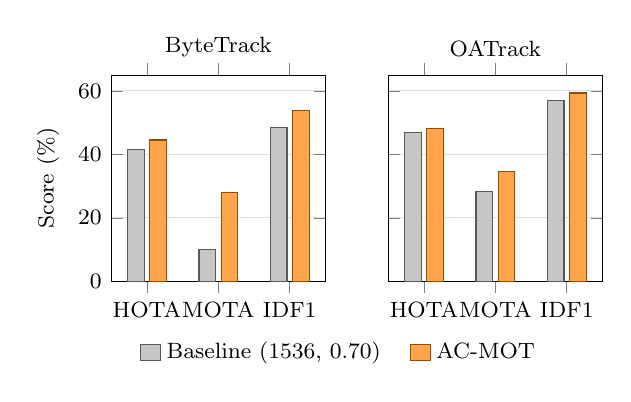
\begin{tikzpicture}
\begin{groupplot}[
  group style={group size=2 by 1, horizontal sep=8mm},
  width=43mm, height=42mm,
  ybar, /pgf/bar width=6pt, ymin=0, ymax=65,
  symbolic x coords={HOTA,MOTA,IDF1}, xtick=data,
  enlarge x limits=0.25,
  ymajorgrids, grid style={gray!25},
  tick label style={font=\footnotesize},
  title style={font=\footnotesize, yshift=-1mm},
  ylabel style={font=\footnotesize},
  legend style={font=\footnotesize, draw=none, legend columns=2,
                at={(1.07,-0.24)}, anchor=north, /tikz/every even column/.append style={column sep=3mm}},
  legend image code/.code={\draw[#1] (0cm,-0.1cm) rectangle (0.25cm,0.1cm);}]
\nextgroupplot[title={ByteTrack}, ylabel={Score (\%)}]
\addplot[fill=gray!45, draw=gray!70!black] coordinates {(HOTA,41.586) (MOTA,9.876) (IDF1,48.569)};
\addplot[fill=orange!70, draw=orange!60!black] coordinates {(HOTA,44.523) (MOTA,27.871) (IDF1,53.929)};
\legend{{Baseline (1536, 0.70)}, {AC-MOT}}
\nextgroupplot[title={OATrack}, yticklabels={}]
\addplot[fill=gray!45, draw=gray!70!black] coordinates {(HOTA,46.770) (MOTA,28.165) (IDF1,57.107)};
\addplot[fill=orange!70, draw=orange!60!black] coordinates {(HOTA,48.095) (MOTA,34.483) (IDF1,59.364)};
\end{groupplot}
\end{tikzpicture}
\caption{HOTA, MOTA, and IDF1 on the seven VisDrone sequences for both
tracker hosts (values in Table~\ref{tab:visdrone}).}
\label{fig:visdrone}
\end{figure}

\begin{table}[htbp]
\caption{Paired sequence-level bootstrap on VisDrone: AC-MOT minus baseline,
5000 resamples, seed 42. HOTA, MOTA, IDF1, precision, and recall in points;
IDS, FP, and FN in counts.}
\label{tab:bootstrap}
\centering\footnotesize
\setlength{\tabcolsep}{4pt}
\begin{tabular}{@{}llrr@{}}
\toprule
Host & Metric & Difference & 95\% interval\\
\midrule
ByteTrack & HOTA & $+2.937$ & $[+2.356, +3.375]$\\
 & MOTA & $+17.995$ & $[+13.541, +23.282]$\\
 & IDF1 & $+5.360$ & $[+4.490, +6.178]$\\
 & IDS & $-325$ & $[-498, -164]$\\
 & FP & $-14382$ & $[-19176, -9620]$\\
 & FN & $+1781$ & $[+288, +3594.075]$\\
 & Precision & $+10.003$ & $[+8.712, +11.895]$\\
 & Recall & $-2.479$ & $[-4.507, -0.469]$\\
\midrule
OATrack & HOTA & $+1.325$ & $[+0.200, +2.264]$\\
 & MOTA & $+6.318$ & $[+4.741, +7.879]$\\
 & IDF1 & $+2.258$ & $[+0.548, +3.474]$\\
 & IDS & $-169$ & $[-292, -42]$\\
 & FP & $-3994$ & $[-6190, -2494.900]$\\
 & FN & $-375$ & $[-1462.575, +670]$\\
 & Precision & $+3.981$ & $[+2.957, +5.511]$\\
 & Recall & $+0.522$ & $[-0.869, +2.111]$\\
\bottomrule
\end{tabular}
\end{table}

\emph{Paired bootstrap.} Table~\ref{tab:bootstrap} gives the paired differences (AC-MOT minus baseline)
and their 95\% intervals. With ByteTrack, the intervals of HOTA, MOTA, IDF1,
precision, IDS, and FP lie entirely on the side of improvement, and FN and
recall move in the opposite direction. With OATrack, HOTA, MOTA, IDF1, and
precision rise and IDS and FP fall, all with intervals on one side of zero.
Because whole sequences are resampled, these intervals reflect the variation
between videos, not only between frames.

\emph{Controller behaviour.} The controller uses all three states with both hosts. With ByteTrack, LOW,
MEDIUM, and HIGH cover 7.4\%, 30.1\%, and 62.5\% of the frames; with OATrack
they cover 7.4\%, 33.3\%, and 59.3\%. For most of the video, the detector
therefore runs with the HIGH action, the smallest input and a score threshold
of 0.40. The two hosts diverge through their different tracked boxes. State changes are rare, between 0.10 and 0.54 per 100
frames depending on the sequence, so the detector input stays stable over
long stretches of video.

\subsection{Frozen UAVDT transfer}
The UAVDT transfer tests whether the frozen controller still helps on a
dataset with other scenes, object types, and recording conditions, when none
of its values is changed. It uses 20 test sequences with 16,592 frames, scored
with one vehicle class. The frozen controller, thresholds, and action map are
applied without any change. Detector outputs for UAVDT were produced at the three
frozen operating points, giving 49,776 detector forward passes. UAVDT is a
single frozen run per host. The paired bootstrap draws 20 sequences with
replacement from these runs. It is computed from the stored per-sequence
counts of the two systems and therefore covers the count-based metrics MOTA,
IDF1, IDS, FP, and FN.

\begin{table}[htbp]
\caption{Frozen UAVDT transfer without retuning (20 sequences, 16,592 frames,
one vehicle class). Baseline: fixed operating point (1536, 0.70).}
\label{tab:uavdt}
\centering\footnotesize
\setlength{\tabcolsep}{4pt}
\begin{tabular}{@{}lrrrr@{}}
\toprule
 & \multicolumn{2}{c}{ByteTrack} & \multicolumn{2}{c}{OATrack}\\
\cmidrule(lr){2-3}\cmidrule(l){4-5}
Metric & Baseline & AC-MOT & Baseline & AC-MOT\\
\midrule
HOTA & 45.923 & 47.004 & 47.728 & 47.640\\
MOTA & $-1.573$ & 16.028 & 19.607 & 22.873\\
IDF1 & 58.400 & 61.767 & 62.101 & 62.931\\
IDS & 601 & 486 & 517 & 486\\
FP & 279616 & 212077 & 197937 & 183669\\
FN & 66050 & 73702 & 75612 & 78774\\
Precision & 49.571 & 55.751 & 57.270 & 58.800\\
Recall & 80.625 & 78.381 & 77.820 & 76.893\\
\bottomrule
\end{tabular}
\end{table}

\begin{table}[htbp]
\caption{Paired sequence-level bootstrap on UAVDT: AC-MOT minus baseline,
5000 resamples, seed 42, 20 sequences. MOTA and IDF1 in points; IDS, FP, and
FN in counts.}
\label{tab:uavdt-boot}
\centering\footnotesize
\setlength{\tabcolsep}{4pt}
\begin{tabular}{@{}llrr@{}}
\toprule
Host & Metric & Difference & 95\% interval\\
\midrule
ByteTrack & MOTA & $+17.601$ & $[+11.134, +26.767]$\\
 & IDF1 & $+3.367$ & $[+1.676, +5.013]$\\
 & IDS & $-115$ & $[-211.025, -26.975]$\\
 & FP & $-67539$ & $[-104215.350, -37352.950]$\\
 & FN & $+7652$ & $[+1542.925, +18359.400]$\\
\midrule
OATrack & MOTA & $+3.267$ & $[+0.607, +5.881]$\\
 & IDF1 & $+0.831$ & $[+0.125, +1.271]$\\
 & IDS & $-31$ & $[-101, +39]$\\
 & FP & $-14268$ & $[-33958.075, -2188.950]$\\
 & FN & $+3162$ & $[-211.100, +8959.050]$\\
\bottomrule
\end{tabular}
\end{table}

Table~\ref{tab:uavdt} and Fig.~\ref{fig:uavdt} report the transfer to UAVDT
without retuning. With ByteTrack, HOTA changes from 45.923 to 47.004 ($+1.081$),
MOTA from $-1.573$ to 16.028 ($+17.601$), and IDF1 from 58.400 to 61.767
($+3.367$). IDS fall by 115 and FP by 67539, while FN rise by 7652. With
OATrack, MOTA changes from 19.607 to 22.873 ($+3.267$), IDF1 from 62.101 to
62.931 ($+0.831$), IDS fall by 31, and FP fall by 14268, while HOTA is almost
unchanged (47.728 and 47.640). With both hosts the transfer gives fewer FP and
IDS and higher precision, with slightly lower recall, the same pattern as with
ByteTrack on VisDrone. The controller therefore changes the detector output in
the same way on a dataset that was not used to build it.

Table~\ref{tab:uavdt-boot} gives the paired bootstrap differences on UAVDT.
With ByteTrack, the intervals of MOTA, IDF1, IDS, and FP lie entirely on the
side of improvement, and FN moves in the opposite direction. With OATrack,
MOTA and IDF1 rise and FP fall, with intervals on one side of zero, while the
intervals of IDS and FN include zero.

\begin{figure}[htbp]
\centering
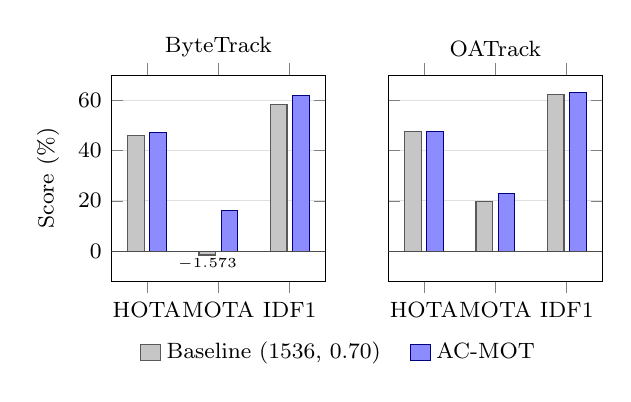
\begin{tikzpicture}
\begin{groupplot}[
  group style={group size=2 by 1, horizontal sep=8mm},
  width=43mm, height=42mm,
  ybar, /pgf/bar width=6pt, ymin=-12, ymax=70, ytick={0,20,40,60},
  symbolic x coords={HOTA,MOTA,IDF1}, xtick=data,
  enlarge x limits=0.25,
  ymajorgrids, grid style={gray!25},
  tick label style={font=\footnotesize},
  title style={font=\footnotesize, yshift=-1mm},
  ylabel style={font=\footnotesize},
  legend style={font=\footnotesize, draw=none, legend columns=2,
                at={(1.07,-0.24)}, anchor=north, /tikz/every even column/.append style={column sep=3mm}},
  legend image code/.code={\draw[#1] (0cm,-0.1cm) rectangle (0.25cm,0.1cm);}]
\nextgroupplot[title={ByteTrack}, ylabel={Score (\%)}]
\addplot[fill=gray!45, draw=gray!70!black] coordinates {(HOTA,45.923) (MOTA,-1.573) (IDF1,58.400)};
\addplot[fill=blue!45, draw=blue!50!black] coordinates {(HOTA,47.004) (MOTA,16.028) (IDF1,61.767)};
\node[font=\tiny, anchor=north, inner sep=1pt, xshift=-4pt] at (axis cs:MOTA,-1.573) {$-1.573$};
\draw[black!70] ({rel axis cs:0,0}|-{axis cs:HOTA,0}) -- ({rel axis cs:1,0}|-{axis cs:HOTA,0});
\legend{{Baseline (1536, 0.70)}, {AC-MOT}}
\nextgroupplot[title={OATrack}, yticklabels={}]
\addplot[fill=gray!45, draw=gray!70!black] coordinates {(HOTA,47.728) (MOTA,19.607) (IDF1,62.101)};
\addplot[fill=blue!45, draw=blue!50!black] coordinates {(HOTA,47.640) (MOTA,22.873) (IDF1,62.931)};
\draw[black!70] ({rel axis cs:0,0}|-{axis cs:HOTA,0}) -- ({rel axis cs:1,0}|-{axis cs:HOTA,0});
\end{groupplot}
\end{tikzpicture}
\caption{HOTA, MOTA, and IDF1 of the frozen UAVDT transfer for both tracker
hosts (values in Table~\ref{tab:uavdt}). The ByteTrack baseline MOTA is
negative ($-1.573$); the solid line marks zero.}
\label{fig:uavdt}
\end{figure}
\section{Discussion}\label{sec:discussion}

\emph{The operating point is part of the MOT system.} The same frozen detector
and the same trackers give very different MOT results at different operating
points. Moving away from the fixed 1536/0.70 point raises MOTA by 17.995 points
with ByteTrack and by 6.318 points with OATrack on VisDrone. The detector
operating point is therefore a first-order variable of aerial MOT and deserves
the same attention as the association method.

\emph{A more selective detection stream.} The main effect of AC-MOT is a more
selective detection stream. FP and IDS drop sharply, precision rises, and FN
rise a little with ByteTrack. MOTA reacts most strongly because it counts FP
directly; HOTA and IDF1 rise by smaller amounts. The same pattern appears on
UAVDT, where FP fall by 67539 with ByteTrack and by 14268 with OATrack.

\emph{Tracker dependence.} ByteTrack gains more than OATrack. ByteTrack starts
from a weaker baseline and uses low-score boxes in its second association
step, so a likely reason is that removing clutter helps it directly. OATrack
already weights detections by quality inside its association, and it gains
mainly in MOTA, IDF1, IDS, and FP. Results are therefore reported per host.

\emph{Development path.} The historical profiles showed that the preferred
operating point depends on the goal: quality or identity stability and speed.
The transfer studies showed that the effect also depends on the tracker host.
The modern stage turned these observations into a finite, readable controller
with one crowd index, a few guard cues, three states, and three actions. Its
cue subset, thresholds, and actions were selected on calibration sequences,
and its results are reported per host.

\emph{Deployment.} AC-MOT needs no training and no access to detector or
tracker internals. It changes three arguments of the detector call. Its
analysis runs on a quarter-scale image every ten frames and uses boxes that
the tracker already produced. On a Tesla T4 the controller takes 4.26 ms per
frame with ByteTrack and 4.20 ms with OATrack, which is small next to detector
inference. The control layer therefore adds very little latency and is
suitable for real-time use. The same interface can host other action maps, for
example maps chosen for a latency budget, without changes to the detector or
the tracker.
\section{Conclusion}\label{sec:conclusion}

This paper presented AC-MOT, a training-free method that adjusts the detector
operating point online to improve MOT in UAV videos. Instead of using fixed
detector settings, AC-MOT changes the confidence threshold, the NMS IoU
threshold, and the input resolution as the scene changes. It uses only the
current frame and previous tracking results, and it does not change or retrain
the detector or the tracker. The SCI, which is based on object density,
together with a few other scene cues and a three-state controller with
recovery, hysteresis, and dwell rules, lets the settings follow the scene
without frequent changes.

The controller was developed through optimization experiments, and its final
values were selected by cross-validation on separate calibration sequences and
then kept fixed.

On seven VisDrone2019-MOT sequences, AC-MOT improved HOTA by 2.937 points with
ByteTrack and 1.325 points with OATrack, and MOTA by 17.995 and 6.318 points,
respectively; paired bootstrap analysis gave confidence intervals for these
differences. On UAVDT, the same controller improved MOTA by 17.601 points with
ByteTrack and 3.267 points with OATrack without retuning.

Overall, the results show that the detector operating point should be treated
as part of the tracking system rather than as a fixed setting. Future work
will test the controller with more detectors, trackers, and aerial video
datasets.

% Bibliography is embedded so that this file compiles on its own.
\begin{thebibliography}{31}
\newcommand{\enquote}[1]{``#1''}
\providecommand{\natexlab}[1]{#1}
\providecommand{\url}[1]{\texttt{#1}}
\providecommand{\urlprefix}{URL }
\expandafter\ifx\csname urlstyle\endcsname\relax
  \providecommand{\doi}[1]{doi:\discretionary{}{}{}#1}\else
  \providecommand{\doi}{doi:\discretionary{}{}{}\begingroup
  \urlstyle{rm}\Url}\fi

\bibitem[{Wu et~al.(2022)Wu, Li, Hong, Tao, and Du}]{wu2022uavsurvey}
Wu, X., Li, W., Hong, D., Tao, R., and Du, Q., \enquote{{Deep Learning for
  Unmanned Aerial Vehicle-Based Object Detection and Tracking: A survey},}
  \emph{IEEE Geoscience and Remote Sensing Magazine}, Vol.~10, No.~1, 2022, pp.
  91--124.
\newblock \doi{10.1109/mgrs.2021.3115137}.

\bibitem[{Zhu et~al.(2022)Zhu, Wen, Du, Bian, Fan, Hu, and
  Ling}]{zhu2022visdrone}
Zhu, P., Wen, L., Du, D., Bian, X., Fan, H., Hu, Q., and Ling, H.,
  \enquote{{Detection and Tracking Meet Drones Challenge},} \emph{IEEE
  Transactions on Pattern Analysis and Machine Intelligence}, Vol.~44, No.~11,
  2022, pp. 7380--7399.
\newblock \doi{10.1109/tpami.2021.3119563}.

\bibitem[{Du et~al.(2018)Du, Qi, Yu, Yang, Duan, Li, Zhang, Huang, and
  Tian}]{du2018uavdt}
Du, D., Qi, Y., Yu, H., Yang, Y., Duan, K., Li, G., Zhang, W., Huang, Q., and
  Tian, Q., \enquote{{The Unmanned Aerial Vehicle Benchmark: Object Detection
  and Tracking},} \emph{Computer Vision -- ECCV 2018}, Springer International
  Publishing, Cham, 2018, pp. 375--391.
\newblock \doi{10.1007/978-3-030-01249-6_23}.

\bibitem[{Cheng et~al.(2023)Cheng, Yuan, Yao, Yan, Zeng, Xie, and
  Han}]{cheng2023smallobject}
Cheng, G., Yuan, X., Yao, X., Yan, K., Zeng, Q., Xie, X., and Han, J.,
  \enquote{{Towards Large-Scale Small Object Detection: Survey and
  Benchmarks},} \emph{IEEE Transactions on Pattern Analysis and Machine
  Intelligence}, 2023, pp. 1--20.
\newblock \doi{10.1109/tpami.2023.3290594}.

\bibitem[{Bewley et~al.(2016)Bewley, Ge, Ott, Ramos, and
  Upcroft}]{bewley2016sort}
Bewley, A., Ge, Z., Ott, L., Ramos, F., and Upcroft, B., \enquote{{Simple
  online and realtime tracking},} \emph{2016 IEEE International Conference on
  Image Processing (ICIP)}, IEEE, Phoenix, AZ, USA, 2016, pp. 3464--3468.
\newblock \doi{10.1109/icip.2016.7533003}.

\bibitem[{Zhang et~al.(2022)Zhang, Sun, Jiang, Yu, Weng, Yuan, Luo, Liu, and
  Wang}]{zhang2022bytetrack}
Zhang, Y., Sun, P., Jiang, Y., Yu, D., Weng, F., Yuan, Z., Luo, P., Liu, W.,
  and Wang, X., \enquote{{ByteTrack: Multi-object Tracking by Associating Every
  Detection Box},} \emph{Computer Vision -- ECCV 2022}, Springer Nature
  Switzerland, Cham, 2022, pp. 1--21.
\newblock \doi{10.1007/978-3-031-20047-2_1}.

\bibitem[{Chin et~al.(2019)Chin, Ding, and Marculescu}]{chin2019adascale}
Chin, T.-W., Ding, R., and Marculescu, D., \enquote{{AdaScale: Towards
  Real-time Video Object Detection using Adaptive Scaling},} \emph{Proceedings
  of Machine Learning and Systems}, Vol.~1, 2019, pp. 431--441.

\bibitem[{Xu et~al.(2020)Xu, lin Zhang, Wang, Lee, Mitra, Chaterji, Li, and
  Bagchi}]{xu2020approxdet}
Xu, R., lin Zhang, C., Wang, P., Lee, J., Mitra, S., Chaterji, S., Li, Y., and
  Bagchi, S., \enquote{{ApproxDet: Content and Contention-Aware Approximate
  Object Detection for Mobiles},} \emph{Proceedings of the 18th Conference on
  Embedded Networked Sensor Systems (SenSys)}, ACM, 2020, pp. 449--462.
\newblock \doi{10.1145/3384419.3431159}.

\bibitem[{Ma et~al.(2023)Ma, Hussain, Park, Kim, and
  Jeon}]{ma2023adaptivebytetrack}
Ma, L.~V., Hussain, M.~I., Park, J., Kim, J., and Jeon, M., \enquote{{Adaptive
  Confidence Threshold for ByteTrack in Multi-Object Tracking},} \emph{2023
  12th International Conference on Control, Automation and Information Sciences
  (ICCAIS)}, IEEE, 2023, pp. 370--374.
\newblock \doi{10.1109/iccais59597.2023.10382403}.

\bibitem[{Shim et~al.(2024)Shim, Ko, Hwang, and Kim}]{shim2024adaptrack}
Shim, K., Ko, K., Hwang, J., and Kim, C., \enquote{{AdapTrack: Adaptive
  Thresholding-Based Matching for Multi-Object Tracking},} \emph{2024 IEEE
  International Conference on Image Processing (ICIP)}, IEEE, 2024, pp.
  2222--2228.
\newblock \doi{10.1109/icip51287.2024.10648139}.

\bibitem[{Dendorfer et~al.(2021)Dendorfer, O{\v{s}}ep, Milan, Schindler,
  Cremers, Reid, Roth, and Leal-Taix{\'e}}]{dendorfer2021motchallenge}
Dendorfer, P., O{\v{s}}ep, A., Milan, A., Schindler, K., Cremers, D., Reid, I.,
  Roth, S., and Leal-Taix{\'e}, L., \enquote{{MOTChallenge: A Benchmark for
  Single-Camera Multiple Target Tracking},} \emph{International Journal of
  Computer Vision}, Vol. 129, No.~4, 2021, pp. 845--881.
\newblock \doi{10.1007/s11263-020-01393-0}.

\bibitem[{Luiten et~al.(2021)Luiten, O\v{s}ep, Dendorfer, Torr, Geiger,
  Leal-Taix\'{e}, and Leibe}]{luiten2021hota}
Luiten, J., O\v{s}ep, A., Dendorfer, P., Torr, P., Geiger, A., Leal-Taix\'{e},
  L., and Leibe, B., \enquote{{HOTA: A Higher Order Metric for Evaluating
  Multi-object Tracking},} \emph{International Journal of Computer Vision},
  Vol. 129, No.~2, 2021, pp. 548--578.
\newblock \doi{10.1007/s11263-020-01375-2}.

\bibitem[{Efron and Tibshirani(1993)}]{efron1993bootstrap}
Efron, B., and Tibshirani, R.~J., \emph{An Introduction to the Bootstrap},
  Springer US, New York, 1993.
\newblock \doi{10.1007/978-1-4899-4541-9}.

\bibitem[{Du et~al.(2023)Du, Zhao, Song, Zhao, Su, Gong, and
  Meng}]{du2023strongsort}
Du, Y., Zhao, Z., Song, Y., Zhao, Y., Su, F., Gong, T., and Meng, H.,
  \enquote{{StrongSORT: Make DeepSORT Great Again},} \emph{IEEE Transactions on
  Multimedia}, Vol.~25, 2023, pp. 8725--8737.
\newblock \doi{10.1109/tmm.2023.3240881}.

\bibitem[{Meinhardt et~al.(2022)Meinhardt, Kirillov, Leal-Taixe, and
  Feichtenhofer}]{meinhardt2022trackformer}
Meinhardt, T., Kirillov, A., Leal-Taixe, L., and Feichtenhofer, C.,
  \enquote{{TrackFormer: Multi-Object Tracking With Transformers},}
  \emph{Proceedings of the IEEE/CVF Conference on Computer Vision and Pattern
  Recognition (CVPR)}, 2022, pp. 8844--8854.

\bibitem[{Liu et~al.(2022)Liu, Li, Lu, and He}]{liu2022uavmot}
Liu, S., Li, X., Lu, H., and He, Y., \enquote{{Multi-Object Tracking Meets
  Moving UAV},} \emph{2022 IEEE/CVF Conference on Computer Vision and Pattern
  Recognition (CVPR)}, IEEE, 2022, pp. 8866--8875.
\newblock \doi{10.1109/cvpr52688.2022.00867}.

\bibitem[{Miller and Rogers(2015)}]{miller2015multitarget}
Miller, N., and Rogers, J., \enquote{{Simultaneous Tracking of Multiple Ground
  Targets from a Multirotor Unmanned Aerial Vehicle},} \emph{Journal of
  Aerospace Information Systems}, Vol.~12, No.~3, 2015, pp. 345--364.
\newblock \doi{10.2514/1.i010345}.

\bibitem[{Desai and Lee(2017)}]{desai2017uavfeature}
Desai, A., and Lee, D.-J., \enquote{{Efficient Feature Descriptor for Unmanned
  Aerial Vehicle Ground Moving Object Tracking},} \emph{Journal of Aerospace
  Information Systems}, Vol.~14, No.~6, 2017, pp. 345--350.
\newblock \doi{10.2514/1.i010503}.

\bibitem[{Lu and Sun(2024)}]{lu2024uavdetection}
Lu, Y.-R., and Sun, D., \enquote{{Development of Real-Time Unmanned Aerial
  Vehicle Urban Object Detection System with Federated Learning},}
  \emph{Journal of Aerospace Information Systems}, Vol.~21, No.~7, 2024, pp.
  547--553.
\newblock \doi{10.2514/1.i011378}.

\bibitem[{Choi et~al.(2022)Choi, Park, and Han}]{choi2022docking}
Choi, A.~J., Park, J., and Han, J.-H., \enquote{{Automated Aerial Docking
  System Using Onboard Vision-Based Deep Learning},} \emph{Journal of Aerospace
  Information Systems}, Vol.~19, No.~6, 2022, pp. 421--436.
\newblock \doi{10.2514/1.i011053}.

\bibitem[{Dai et~al.(2026)Dai, Chen, Lian, and Xie}]{dai2026lsoyolo}
Dai, P., Chen, L., Lian, Y., and Xie, L., \enquote{{LSO-YOLO: a lightweight
  real-time object detection network for UAV small-object detection},}
  \emph{Journal of Real-Time Image Processing}, Vol.~23, No.~5, 2026, p. 176.
\newblock \doi{10.1007/s11554-026-01977-y}.

\bibitem[{Qi et~al.(2026)Qi, Wang, and Jiang}]{qi2026oatrack}
Qi, L., Wang, L., and Jiang, S., \enquote{{OATrack: A Quality-Gated Progressive
  Association Framework with a YOLO Detection Cache for UAV Small-Object
  Multi-Object Tracking},} \emph{Sensors}, Vol.~26, No.~16, 2026, p. 5222.
\newblock \doi{10.3390/s26165222}.

\bibitem[{Jocher and Qiu(2024)}]{jocher2024yolo11}
Jocher, G., and Qiu, J., \enquote{{Ultralytics YOLO11},}
  \url{https://github.com/ultralytics/ultralytics}, 2024.
\newblock Version 11.0.0.

\bibitem[{Han et~al.(2022)Han, Huang, Song, Yang, Wang, and
  Wang}]{han2022dynamic}
Han, Y., Huang, G., Song, S., Yang, L., Wang, H., and Wang, Y.,
  \enquote{{Dynamic Neural Networks: A Survey},} \emph{IEEE Transactions on
  Pattern Analysis and Machine Intelligence}, Vol.~44, No.~11, 2022, pp.
  7436--7456.
\newblock \doi{10.1109/tpami.2021.3117837}.

\bibitem[{Yang et~al.(2020)Yang, Han, Chen, Song, Dai, and
  Huang}]{yang2020ranet}
Yang, L., Han, Y., Chen, X., Song, S., Dai, J., and Huang, G.,
  \enquote{{Resolution Adaptive Networks for Efficient Inference},}
  \emph{Proceedings of the IEEE/CVF Conference on Computer Vision and Pattern
  Recognition (CVPR)}, 2020, pp. 2369--2378.

\bibitem[{Jiang et~al.(2018)Jiang, Ananthanarayanan, Bodik, Sen, and
  Stoica}]{jiang2018chameleon}
Jiang, J., Ananthanarayanan, G., Bodik, P., Sen, S., and Stoica, I.,
  \enquote{{Chameleon: Scalable Adaptation of Video Analytics},}
  \emph{Proceedings of the 2018 Conference of the ACM Special Interest Group on
  Data Communication}, ACM, New York, NY, USA, 2018, pp. 253--266.
\newblock \doi{10.1145/3230543.3230574}.

\bibitem[{Akiba et~al.(2019)Akiba, Sano, Yanase, Ohta, and
  Koyama}]{akiba2019optuna}
Akiba, T., Sano, S., Yanase, T., Ohta, T., and Koyama, M., \enquote{{Optuna: A
  Next-generation Hyperparameter Optimization Framework},} \emph{Proceedings of
  the 25th ACM SIGKDD International Conference on Knowledge Discovery and Data
  Mining}, ACM, Anchorage, AK, USA, 2019, pp. 2623--2631.
\newblock \doi{10.1145/3292500.3330701}.

\bibitem[{Lin et~al.(2014)Lin, Maire, Belongie, Hays, Perona, Ramanan,
  Doll{\'a}r, and Zitnick}]{lin2014coco}
Lin, T.-Y., Maire, M., Belongie, S., Hays, J., Perona, P., Ramanan, D.,
  Doll{\'a}r, P., and Zitnick, C.~L., \enquote{{Microsoft COCO: Common Objects
  in Context},} \emph{Computer Vision -- ECCV 2014}, Springer International
  Publishing, Cham, 2014, pp. 740--755.
\newblock \doi{10.1007/978-3-319-10602-1_48}.

\bibitem[{Jocher et~al.(2023)Jocher, Chaurasia, and Qiu}]{jocher2023yolov8}
Jocher, G., Chaurasia, A., and Qiu, J., \enquote{{Ultralytics YOLOv8},}
  \url{https://github.com/ultralytics/ultralytics}, 2023.
\newblock Version 8.0.0.

\bibitem[{Liu et~al.(2023)Liu, Jin, Fu, Chen, Jiang, and Ye}]{liu2023u2mot}
Liu, K., Jin, S., Fu, Z., Chen, Z., Jiang, R., and Ye, J.,
  \enquote{{Uncertainty-aware Unsupervised Multi-Object Tracking},}
  \emph{Proceedings of the IEEE/CVF International Conference on Computer Vision
  (ICCV)}, 2023, pp. 9996--10005.

\bibitem[{Liu et~al.(2025)Liu, Wang, Wang, Liu, and Bai}]{liu2025sparsetrack}
Liu, Z., Wang, X., Wang, C., Liu, W., and Bai, X., \enquote{{SparseTrack:
  Multi-Object Tracking by Performing Scene Decomposition Based on
  Pseudo-Depth},} \emph{IEEE Transactions on Circuits and Systems for Video
  Technology}, Vol.~35, No.~5, 2025, pp. 4870--4882.
\newblock \doi{10.1109/TCSVT.2024.3524670}.

\end{thebibliography}

\end{document}
